% Modified 31 Oct 2005:  Conditioning fallacy alluded to.
% This chapter has been modified on 6-4-05.
% There are two \choice
\pagestyle{headings}
\chapter{Confidence Intervals \& Hypothesis Tests} \label{chp 5}

%TODO: Examples and discussion of non-CLT confidence intervals.

\section{Confidence Interval for a Population Mean}\index{Confidence Interval! for a Mean}


\subsection*{Estimating Average Age}

In this chapter, we'll put the central limit theorem to work. Suppose we're interested in knowing the mean age of students at Champlain College. To estimate it, we take a random sample of 50 students and record their ages. It turns out that the mean age of students in the sample is $18.3$ years.

Since the sample mean, $\littlexbar = 18.3$, is the mean of a random sample of a sufficiently large size, the central limit theorem tells us $\xbar \sim AG(\muxbar, \sigmaxbar)$. Standardizing the sample mean we observed yields
$$z = \frac{\overline{x} - \muxbar}{\sigmaxbar} = \frac{18.3 - \muxbar}{\sigmaxbar}.$$
Now suppose we happen to know that the standard deviation for ages of students at Champlain College is $2.7$ years. Then since $\muxbar = \mu$ and $\sigmaxbar = \sigma / \sqrt{n} = 2.7 / \sqrt{50} \simeq 0.381$, we can write
$$z = \frac{\overline{x}  - \muxbar}{\sigmaxbar} = \frac{18.3 - \muxbar}{\sigmaxbar} = \frac{18.3 - \mu}{0.381}.$$
We've seen in Proposition \ref{GaussianRuleThumb} that approximately $95\%$ of all values of $Z$ fall into the interval $(-2, 2)$, and hence we should be about 95\% confident that
\begin{gather*}
-2 < \textstyle\frac{18.3 - \mu}{0.381} < 2 \\
-0.762 < 18.3 - \mu < 0.762 \\
-19.062 < - \mu < -17.538 \\
17.538 < \mu < 19.062.
\end{gather*}

This range of values is called a \index{Confidence Interval}\newterm{confidence interval} for the parameter $\mu$, which in this case represents the mean age of all students at Champlain College. We can't determine the exact value of $\mu$ without collecting information from every single student. However, from one random sample of fifty students, we can assert that $17.5 < \mu < 19.1$ with 95\% confidence.

Confidence intervals are so useful and pervasive in applications of statistics, it's worth our while to set up some notation and terminology to make constructing them as routine as possible.

\begin{definition}\index{Critical Value}\index{Confidence Level}Given a confidence level $C \in (0,1)$, the \newterm{critical value} corresponding to that confidence level is the value $z^*$ with $P(-z^* < Z < z^*) = C$.
\end{definition}
\begin{center}
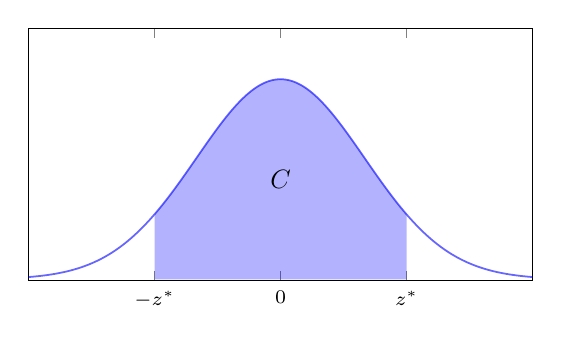
\begin{tikzpicture}[scale = 0.8]
  \begin{axis}[
  	  scale only axis,
      tick label style={font=\scriptsize, scale = 1/0.8},
      width = 8cm,
      height = 4cm,
      ymin=-0.0025,
      ymax=0.5,
      xmin=-3,
      xmax=3,
      xtick = {-1.5,0,1.5}, xticklabels = {$-z^*$,$0$,$z^*$},
      ytick=\empty,
      legend pos=north east,
      domain=-3:3,
      samples=200,
      thick
    ]
    \addplot[blue,opacity=0.6] {0.3989*pow(e,-x^2/2)};
    \addplot[blue, opacity=0, fill=blue, fill opacity=0.3, domain=-1.5:1.5] 
      {0.3989*pow(e,-x^2/2)}\closedcycle;
    \node at (axis cs: 0,0.2) {\large{$C$}};
  \end{axis}
\end{tikzpicture}
\end{center}

\begin{example}
The critical value for a confidence level of $90\%$ is $z^* = 1.65$, since 
$$P(-1.65 < Z < 1.65) = P(Z < 1.65) - P(Z < -1.65) = 0.9505 - 0.495 = 0.9.$$
\begin{center}
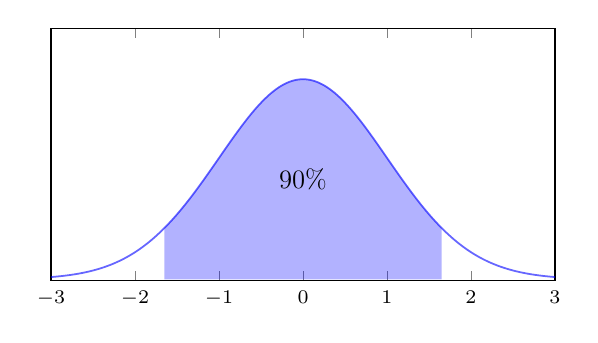
\begin{tikzpicture}[scale = 0.8]
  \begin{axis}[
  	  scale only axis,
      tick label style={font=\scriptsize, scale = 1/0.8},
      width = 8cm,
      height = 4cm,
      ymin=-0.0025,
      ymax=0.5,
      xmin=-3,
      xmax=3,
      xtick={-3,-2,-1,0,1,2,3},
      ytick=\empty,
      legend pos=north east,
      domain=-3:3,
      samples=200,
      thick
    ]   
    \addplot[blue,opacity=0.6] {0.3989*pow(e,-x^2/2)}; 
    \addplot[blue, opacity=0, fill=blue, fill opacity=0.3, domain=-1.65:1.65] 
      {0.3989*pow(e,-x^2/2)}\closedcycle;   
    \node at (axis cs: 0,0.2) {\large{$90\%$}};
  \end{axis}
\end{tikzpicture}
\end{center}
Using the $Z$-table, we can find $z^*$ by noting that if $P(-z^* < Z < z^*) = 0.9$, then by symmetry, the area in both tails is 0.05, so $P(Z < z^*) = 0.95$. Thus, we're looking for the value of $z$ that has an area of 0.95 to its left.
\end{example}

If we repeat the calculation we made in the introduction to this section, but this time with a general critical value $z^*$ and sample mean $\xbar$, we'll arrive at a general formula for a confidence interval for the mean $\mu$ of any population from which we might draw a sample. With a probability of $C$, we have
\begin{gather*}
-z^* < Z < z^* \\
-z^* < \textstyle\frac{\overline{X}- \muxbar}{\sigmaxbar} < z^* \\
-z^* \sigmaxbar < \overline{X}- \mu < z^* \sigmaxbar \\[0.2ex]
-\overline{X}-z^* \sigmaxbar < - \mu < -\overline{X}+z^* \sigmaxbar \\[0.3ex]
\overline{X}-z^* \sigmaxbar <  \mu < \overline{X}+z^* \sigmaxbar \\[0.3ex]
\overline{X}-z^* \textstyle\frac{\sigma}{\sqrt{n}} <  \mu < \overline{X}+z^* 
\frac{\sigma}{\sqrt{n}}.
\end{gather*}

This result here only holds if $\xbar$ is Gaussian, but the central limit theorem assures us that as long as our data comes from a random sample of sufficiently large size, we are justified in treating it as such. The quantity we add to and subtract from $\xbar$ in the last line is called the margin of error.

\begin{definition}\index{Margin of Error! for a Mean} Given a random sample of $n$ values drawn from a distribution with standard deviation $\sigma$, and a confidence level $C \in (0,1)$, the \newterm{margin of error} for $\overline{X}$ at confidence level $C$ is 
$$E = z^* \frac{\sigma}{\sqrt{n}}$$
\end{definition}

This value represents the largest possible gap between a sample mean $\overline{X}$ and the population mean $\mu$ that is observed at the confidence level $C$. For example, if $E = 2$ when $C = 0.9$, this means that 90\% of random samples have means which differ from the population mean by less than $2$.

With these definitions established, we can describe the procedure for constructing a confidence interval for a population mean $\mu$ based on a random sample of $n$ values with mean $\littlexbar$ in three steps.
\begin{enumerate}[label=\textnormal{\Roman*}.]
\item Find the critical value $z^*$ for the desired confidence level $C$.
\item Compute the margin of error $E$.
\item The confidence interval is given by $\littlexbar - E < \mu < \littlexbar + E$.
\end{enumerate}

\begin{example} 
The standard deviation for heights of all men in Canada is known to be around 2.9 inches. In a random sample of 37 Canadian men, the average height was 5'9". Use this information to construct a $95\%$ confidence interval for the average height of all Canadian men.
\begin{enumerate}[label=\textnormal{\Roman*}.]
\item The critical value $z^*$ is defined by $P(-z^* < Z < z^*) = 0.95$, so the area on the left of $z^*$ must be $P(Z < z^*) = 0.975$, and consulting the Z-table yields $z^* = 1.96$.
\begin{center}
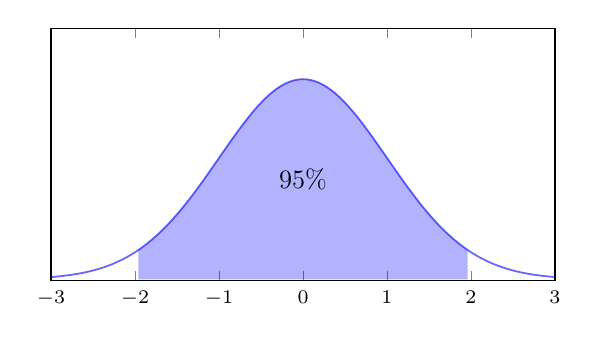
\begin{tikzpicture}[scale = 0.8]
  \begin{axis}[
  	  scale only axis,
      tick label style={font=\scriptsize, scale = 1/0.8},
      width = 8cm,
      height = 4cm,
      ymin=-0.0025,
      ymax=0.5,
      xmin=-3,
      xmax=3,
      xtick={-3,-2,-1,0,1,2,3},
      ytick=\empty,
      legend pos=north east,
      domain=-3:3,
      samples=200,
      thick
    ]
    \addplot[blue,opacity=0.6] {0.3989*pow(e,-x^2/2)};
    \addplot[blue, opacity=0, fill=blue, fill opacity=0.3, domain=-1.96:1.96] 
      {0.3989*pow(e,-x^2/2)}\closedcycle;
    \node at (axis cs: 0,0.2) {\large{$95\%$}}; 
  \end{axis}
\end{tikzpicture}
\end{center}
\item The margin of error is then given by $E = z^*  \frac{\sigma}{\sqrt{n}} = 1.96  \frac{2.9}{\sqrt{37}} \simeq 0.934$. 
\item In inches, the sample mean 5'9" is 69". Adding and subtracting the margin of error gives
$$\begin{aligned}69-0.934 < \ &\mu < 69+0.934 \\
68.066 < \ &\mu < 69.934.\end{aligned}$$
Thus, with $95\%$ confidence, the mean height of all Canadian men must be between 68.066" (about 5'8") and and 69.934" (about 5'10").
\end{enumerate}
\end{example}

Note that when we say `\,with 95\% confidence, $68.066 < \mu < 69.934$\,', this means there is a 95\% chance that we have selected a sample which will produce a confidence interval containing the true mean height of the population, $\mu$.

The mean height of all Canadian men is some fixed single value, we just don't know what it is. Thus, the probability it's inside our particular confidence interval is either $100\%$ or $0\%$ (it is or it isn't, there's no randomness involved). But if we were to take many random samples and compute a 95\% confidence interval from each, we would expect that, typically, nineteen of every twenty samples would produce intervals that contain the true value of $\mu$ (since 19/20 is 95\%). This is the correct interpretation of the confidence level.
\begin{center}
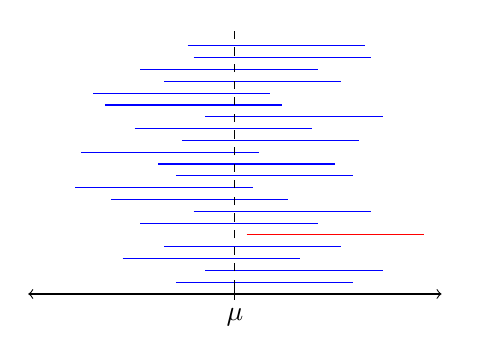
\begin{tikzpicture}[scale=0.75]
\draw[<->] (-3.5,0) -- (3.5,0);
\draw (0,0.1) -- (0,-0.1);
\node at (3.5,-0.4) {};
\node at (0,-0.4) {$\mu$};
\draw[blue] (-1,0.2) -- (2,0.2);
\draw[blue] (-0.5,0.4) -- (2.5,0.4);
\draw[blue] (-1.9,0.6) -- (1.1,0.6);
\draw[blue] (-1.2,0.8) -- (1.8,0.8);
\draw[red] (0.2,1.0) -- (3.2,1.0);
\draw[blue] (-1.6,1.2) -- (1.4,1.2);
\draw[blue] (-0.7,1.4) -- (2.3,1.4);
\draw[blue] (-2.1,1.6) -- (0.9,1.6);
\draw[blue] (-2.7,1.8) -- (0.3,1.8);
\draw[blue] (-1,2.0) -- (2,2.0);
\draw[blue] (-1.3,2.2) -- (1.7,2.2);
\draw[blue] (-2.6,2.4) -- (0.4,2.4);
\draw[blue] (-0.9,2.6) -- (2.1,2.6);
\draw[blue] (-1.7,2.8) -- (1.3,2.8);
\draw[blue] (-0.5,3.0) -- (2.5,3.0);
\draw[blue] (-2.2,3.2) -- (0.8,3.2);
\draw[blue] (-2.4,3.4) -- (0.6,3.4);
\draw[blue] (-1.2,3.6) -- (1.8,3.6);
\draw[blue] (-1.6,3.8) -- (1.4,3.8);
\draw[blue] (-0.7,4.0) -- (2.3,4.0);
\draw[blue] (-0.8,4.2) -- (2.2,4.2);
\draw[dashed] (0,0.1) -- (0,4.5);
\end{tikzpicture}
\end{center}

Notice that as the confidence level becomes larger, the corresponding critical value $z^*$ grows to enclose that larger area, which increases the margin of error, $E$. On the other hand, the value of $E$ is a decreasing function of the sample size, $n$, so a larger sample will lead to a smaller confidence interval, giving a more accurate estimate of the parameter $\mu$.
\begin{prop} To reduce the margin of error $E$ and produce tighter bounds on $\mu$, we can either decrease the confidence level $C$, or increase the sample size $n$.
\end{prop}

Our procedure for constructing a confidence interval for a population mean $\mu$ requires knowledge of the population standard deviation $\sigma$. This is to be expected, as means of samples from a population with a large standard deviation will be more variable than means of samples from a population with a low standard deviation. Unfortunately, this requirement is problematic since $\sigma$ is a parameter of the population distribution, so is almost always unknown in practice.

\subsection*{What if we don't know $\sigma$?}

Can we somehow estimate $\sigma$ and build this estimation process into the confidence interval procedure? The best estimate of the population distribution we have access to is the distribution of values within our sample, so what if we simply use the standard deviation of our sample in place of the standard deviation of the population?

If we use the sample standard deviation, $S$, to estimate the standard deviation in our population, $\sigma$, then when we standardize a sample mean $\xbar$, instead of the standardized value
$$\frac{\overline{X} - \muxbar}{\sigmaxbar} = \frac{\overline{X} - \mu}{\frac{\sigma}{\sqrt{n}}}, \ \ \text{we'll have the estimate} \ \ \frac{\overline{X} - \muxbar}{\sigmaxbar} \approx \frac{\overline{X} - \mu}{\frac{S}{\sqrt{n}}}.$$
Our construction of a confidence interval for the population mean $\mu$ was justified by the central limit theorem, which tells us the distribution of the quantity on the left approaches $Z \sim \Gaussian(0,1)$ as the sample size $n$ grows. But what about our estimate on the right? If we repeatedly draw samples and calculate this value, what kind of distribution will we obtain?

\begin{definition}\label{TDistDef}\index{Distribution! Student's T}\index{T-distribution} Draw a random sample $X_1, X_2, \, \dots \, , X_n$ from a Gaussian distribution with mean $\mu$. Let
$$T = \frac{\overline{X} - \mu}{\frac{S}{\sqrt{n}}}$$
where $S$ is the sample standard deviation, as in Definition \ref{SampleStdDev}. Then $T$ is a continuous random variable whose distribution is called \newterm{Student's $\boldsymbol{T}$-distribution} (or simply the $T$-distribution) with $n-1$ degrees of freedom.
\end{definition}
\begin{center}
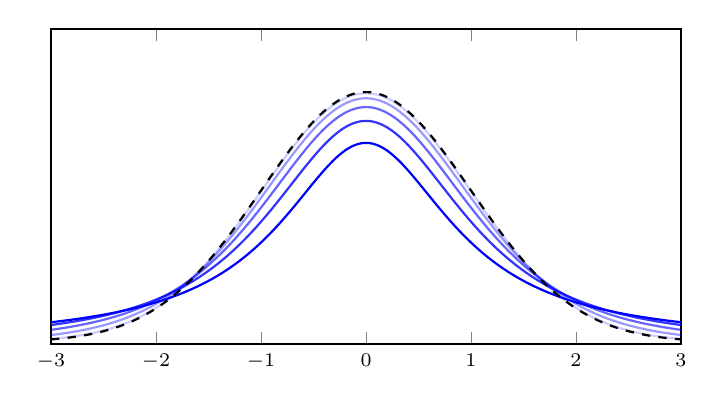
\begin{tikzpicture}[scale = 1]
  \begin{axis}[
  	  scale only axis,
      tick label style={font=\scriptsize, scale = 1},
      width = 8cm,
      height = 4cm,
      ymin=-0.0025,
      ymax=0.5,
      xmin=-3,
      xmax=3,
      xtick={-3,-2,-1,0,1,2,3},
      ytick=\empty,
      legend pos=north east,
      domain=-3:3,
      samples=200,
      thick
    ]
    
    \addplot[blue,opacity=1] {0.318*pow(1+x*x,-1)};
    \addplot[blue,opacity=0.8] {0.353*pow(1+(0.5)*x*x,-1.5)};
    \addplot[blue,opacity=0.6] {0.375*pow(1+(0.25)*x*x,-(0.5*(4+1)))};
    \addplot[blue,opacity=0.4] {0.389*pow(1+(0.1)*x*x,-(0.5*(10+1)))};
    \addplot[blue,opacity=0.2] {0.397*pow(1+(0.01)*x*x,-(0.5*(100+1)))};
    \addplot[black,dashed] {0.3989*pow(e,-x^2/2)};
    
  \end{axis}
\end{tikzpicture}
\end{center}

Above in blue are plots of probability density functions for $T$-distributions with one, two, four, ten, and one hundred degrees of freedom, shaded lighter as the degree of freedom grows. The standard normal distribution is shown in dashed black.

The $T$-distribution has fatter tails and less area near the center than the standard normal distribution. This additional variability appears because the sample standard deviation $S$ differs from one sample to the next, which adds a source of variability to $T$-scores which is not present in $Z$-scores. As the sample size grows, the sample standard deviation $S$ becomes a better estimator of the population standard deviation $\sigma$, and the $T$-distribution slowly approaches the standard normal distribution. Notice that once the degree of freedom reaches one hundred, the $T$-distribution and the standard normal distribution are effectively indistinguishable.

If we can find areas under the $T$-distribution, then the same procedure we've been using to construct confidence intervals with the population standard deviation can be modified to work with the sample standard deviation.

\begin{proposition} Let $\xbar$ and $S$ be the sample mean and (Bessel-corrected) sample standard deviation in a random sample of $n$ values drawn from a Gaussian distribution with mean $\mu$. 

Take $t^*$ such that $P(-t^* < T < t^*) = C$, and let $E = t^*\frac{S}{\sqrt{n}}$. Then $P(\xbar - E < \mu < \xbar + E) = C$.
\end{proposition}
\begin{proofnobox}
By definition of $t^*$, with probability $C$ we have
\begin{gather*}
-t^* < T < t^* \\
-t^* < \textstyle\frac{\overline{X}- \mu}{\frac{S}{\sqrt{n}}} < t^* \\
-t^* \textstyle\frac{S}{\sqrt{n}} < \overline{X}- \mu < t^* \frac{S}{\sqrt{n}} \\[0.2ex]
-\overline{X}-t^* \textstyle\frac{S}{\sqrt{n}} < - \mu < -\overline{X}+t^* \frac{S}{\sqrt{n}} \\[0.3ex]
\overline{X}-t^* \textstyle\frac{S}{\sqrt{n}} <  \mu < \overline{X}+t^* \frac{S}{\sqrt{n}}.
\end{gather*}
\end{proofnobox}

\begin{example}\label{TIntExample} A sample of five values is drawn from a Gaussian distribution with unknown mean and standard deviation. These values are $43$, $27$, $30$, $22$, and $38$. Construct a 90\% confidence interval for the mean of the Gaussian distribution.

Computing the mean and (Bessel corrected) standard deviation of the sample yields $\littlexbar = 32$ and $s = 8.456$. We can now construct a confidence interval for the population mean $\mu$ just as we've done before in the last section, but using $s$ in place of $\sigma$ and the $T$-distribution in place of the standard normal distribution.
%\begin{center}
%   \begin{tikzpicture}[scale = 0.6]
%       \begin{axis}[unit vector ratio=1 6 1, ymin=0,ymax=0.5,xmin=-2.9, xmax = 2.9, xtick = {-2.13,0,2.13}, xticklabels = {$-2.13$,$0$,$2.13$}, ytick = {0.1,0.2,0.3,0.4,0.5}]
%       \addplot[fill = blue, very thick,domain=-2.13:2.13,blue!50, samples=100]  gnuplot {(gamma(0.5*(4+1))/(sqrt(4*pi)*gamma((0.5*4))))*(1+(0.25)*x*x)**(-(0.5*(4+1)))}\closedcycle;
%       \addplot[very thick,domain=-3:3,blue, samples=100]  gnuplot {(gamma(0.5*(4+1))/(sqrt(4*pi)*gamma((0.5*4))))*(1+(0.25)*x*x)**(-(0.5*(4+1)))};
%       \addplot[domain=-3:3] {0};
%       \node at (axis cs: 0,0.2) {\Large{$0.9$}};
%    \end{axis}
%    \end{tikzpicture}
%\end{center}
\begin{center}
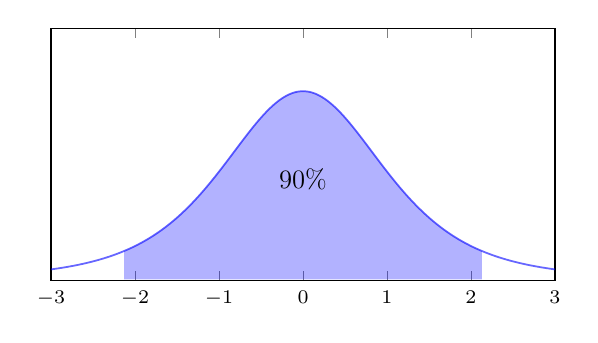
\begin{tikzpicture}[scale = 0.8]
  \begin{axis}[
  	  scale only axis,
      tick label style={font=\scriptsize, scale = 1/0.8},
      width = 8cm,
      height = 4cm,
      ymin=-0.0025,
      ymax=0.5,
      xmin=-3,
      xmax=3,
      xtick={-3,-2,-1,0,1,2,3},
      ytick=\empty,
      legend pos=north east,
      domain=-3:3,
      samples=200,
      thick
    ]
    
    \addplot[blue,opacity=0.6] {0.375*pow(1+(0.25)*x*x,-(0.5*(4+1)))};
    
    \addplot[blue, opacity=0, fill=blue, fill opacity=0.3, domain=-2.13:2.13] 
      {0.375*pow(1+(0.25)*x*x,-(0.5*(4+1)))}\closedcycle;
      
    \node at (axis cs: 0,0.2) {\large{$90\%$}};
    
  \end{axis}
\end{tikzpicture}
\end{center}

\begin{enumerate}[label=\textnormal{\Roman*}.]
\item Using a table of values for the $T$-distribution (with 4 degrees of freedom), we find $t^* = 2.13$.
\item The margin of error is $E = t^{*} \frac{s}{\sqrt{n}} = 2.13 \cdot \frac{8.456}{\sqrt{5}} = 8.05$
\item Therefore, with $90\%$ confidence we have
$$\begin{aligned}32 - 8.05 < \ &\mu < 32 + 8.05 \\
23.95 < \ &\mu < 40.05.\end{aligned}$$
\end{enumerate}
\end{example}

\subsection*{Robustness}\index{Robustness! of $T$-intervals}
Notice that the $T$-distribution is defined as the distribution of $T$-scores of random samples drawn from a Gaussian distribution. In practice though, we would rarely know enough about the population we are studying to be able to determine if the random variable whose mean we want to estimate is Gaussian.

Fortunately, whenever the hypotheses of the central limit theorem hold, the distribution of $T$-scores of random samples will, in fact, eventually converge to the $T$-distribution (which itself converges to the standard normal distribution) as the sample size grows larger, though the justification if this fact is well beyond the scope of this course \cite{vanderVaart}. 

Even with smaller sample sizes, statisticians like to say that the confidence interval procedure above in Example \ref{TIntExample} is `robust to non-normality'. This means that although the assumption that we're sampling from a Gaussian distribution is necessary for the formal justification of the procedure, bending the rules on this assumption will typically only introduce a small source of error. However, with small samples from a population whose distribution is not well understood, one can be justifiably suspicious, especially if there's reason to believe the distribution of the population could be fat-tailed or very asymmetric.

\begin{example}
In a study of a particular species of maple in a provincial park, the height of every tree in a random sample of 38 mature trees was measured. If the sample mean and sample standard deviation for the heights of the trees were $21.3$ metres and $4.9$ metres respectively, construct a $90\%$ confidence interval for the mean height of all trees of this species in the park.

We have a sample of $38$ values with a mean of $\littlexbar = 21.3$ and standard deviation $s = 4.9$.
\begin{center}
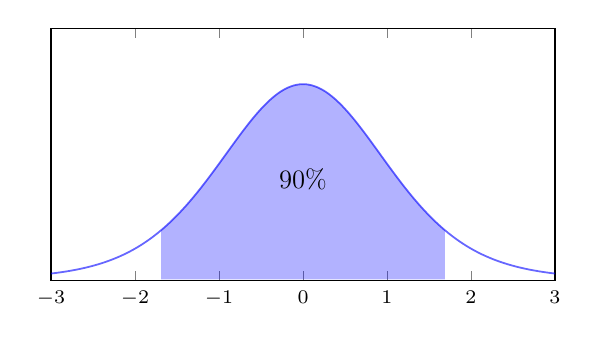
\begin{tikzpicture}[scale = 0.8]
  \begin{axis}[
  	  scale only axis,
      tick label style={font=\scriptsize, scale = 1/0.8},
      width = 8cm,
      height = 4cm,
      ymin=-0.0025,
      ymax=0.5,
      xmin=-3,
      xmax=3,
      xtick={-3,-2,-1,0,1,2,3},
      ytick=\empty,
      legend pos=north east,
      domain=-3:3,
      samples=200,
      thick
    ]
    \addplot[blue,opacity=0.6] {0.389*pow(1+(0.1)*x*x,-(0.5*(10+1)))};
    \addplot[blue, opacity=0, fill=blue, fill opacity=0.3, domain=-1.69:1.69] 
      {0.389*pow(1+(0.1)*x*x,-(0.5*(10+1)))}\closedcycle;
    \node at (axis cs: 0,0.2) {\large{$90\%$}};
  \end{axis}
\end{tikzpicture}
\end{center}
\begin{enumerate}[label=\textnormal{\Roman*}.]
\item Using a table of values for the $T$-distribution (with 37 degrees of freedom), we find $t^* = 1.69$.
\item We can then compute the margin of error $E = t^* \frac{s}{\sqrt{n}} = 1.69 \frac{4.9}{\sqrt{38}} = 1.343$.
\item Thus, with $90\%$ confidence,
$$\begin{aligned}21.3-1.343 < \ &\mu < 21.3+1.343 \\ 
19.957 < \ &\mu < 22.643.\end{aligned}$$
\end{enumerate}
So we conclude that with $90\%$ confidence, the mean height of all mature trees of this species in the park is between $19.9$ and $22.7$ metres.
\end{example}

In contexts like this, where we can be well assured that the distribution our sample is drawn from (the distribution of heights of adult trees of a specific species) is somewhat bell-shaped, and without fat tails, the $T$-distribution confidence interval procedure should hit very close to its target confidence, that is, around 90\% of the intervals constructed at the 90\% confidence level should contain $\mu$.

\begin{keypoint}
We have two variations of the confidence interval procedure for a population mean. In the first, the critical value comes from the standard normal distribution $Z \sim \Gaussian(0,1)$, and in the second it comes from the $T$-distribution with $n-1$ degrees of freedom.

Deciding which variation to use is simple: if the population standard deviation $\sigma$ is known, use the first variation (with $Z$) and if not, use the second (with $T$). 
\end{keypoint}

\begin{remark}
In many treatments of this subject, you'll see that this decision is made on the basis of sample size.

Since the $T$-distribution converges to $Z \sim \Gaussian(0,1)$ as $n \to \infty$, the two variations of the procedure will yield the same interval for large enough samples, so there's an argument to be made that we should use the $Z$-table whenever we can for simplicity's sake. On the other hand, there's also an argument to be made that we should emphasize the distinction between parameters and statistics ($\sigma$ and $S$ in this case) whenever we can, since the easiest way for students to lose their way in statistics is to blur this distinction.
\end{remark}

\section{Confidence Interval for a Population Proportion}\index{Confidence Interval! for a Proportion}

Suppose we're interested in estimating the proportion of individuals in a population that have some property. For example, a pollster might want to estimate the proportion of all voters in a certain riding that intend to vote for a particular political party.

If we randomly select a member of the population and consider selecting someone with the desired property a success, then $X \sim \Bernoulli(p)$ counts the number of successes in a single selection (either zero or one), where the parameter $p$ is the population proportion we want to estimate. The mean of this distribution is $E(X) = p$ (see Section \ref{BernoulliDist}), so the population mean $\mu$ is equal to the population proportion $p$.

When sampling from a Bernoulli distribution, the sample mean $\xbar = \frac{1}{n}(X_1+X_2+\cdots+X_n)$ is the proportion of individuals in the sample that have the desired property ($X_i$ takes the value $1$ when the $i^{th}$ individual has the property, and $0$ if not). Thus, the sample mean $\xbar$ is equal to the sample proportion, which we'll write as $\widehat{p}$.

In summary, if we sample from $X \sim \Bernoulli(p)$, then the population mean and sample mean are equal to the population proportion and sample proportion respectively. This means we can construct a confidence interval for a proportion in exactly the same way we made a confidence interval for a mean in the last section. We're simply applying the same procedure in the special case where our sample is drawn from a Bernoulli distribution.

To produce a confidence interval, we'll need to know, or have to estimate, the standard deviation $\sigma$ of the distribution we're sampling from. For a Bernoulli distribution, this quantity depends completely on the unknown parameter $p$. To be precise, we saw that $\sigma = \sqrt{p(1-p)}$ in Section \ref{BernoulliDist}. Using the sample proportion $\widehat{p}$ in place of the population proportion $p$ gives the estimate $\sqrt{\widehat{p}(1-\widehat{p})}$ for $\sigma$, and applying this estimate in our original margin of error formula for a mean,
$$E = z^{*}\frac{\sigma}{\sqrt{n}}  \ \ \longrightarrow \ \ E = z^{*}\sqrt{\frac{\widehat{p}(1-\widehat{p})}{n}} .$$

We can now construct confidence intervals for proportions using the same three-step procedure we use for means, but with this new margin of error formula.

\begin{example}Suppose that a pollster is interested in knowing what proportion of voters in a certain riding plan to vote NDP. In a random sample of 817 voters from this riding, 227 plan to vote NDP. Construct a $92\%$ confidence interval for the proportion of all voters in this riding who plan to vote NDP.

We have a sample of $817$ values with a sample proportion of $\widehat{p} = \frac{227}{817} = 0.278$. To create a confidence interval for the proportion of NDP voters in the riding, we follow the same three-step procedure as before.
\begin{center}
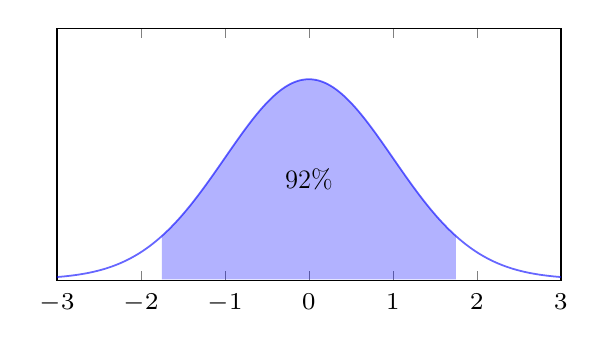
\begin{tikzpicture}[scale = 0.8]
  \begin{axis}[
  	  scale only axis,
      tick label style={font=\scriptsize, scale = 1/0.8},
      width = 8cm,
      height = 4cm,
      ymin=-0.0025,
      ymax=0.5,
      xmin=-3,
      xmax=3,
      tick label style={font=\scriptsize, scale = 1/0.8},
      xtick={-3,-2,-1,0,1,2,3},
      ytick=\empty,
      legend pos=north east,
      domain=-3:3,
      samples=200,
      thick
    ]
    \addplot[blue,opacity=0.6] {0.3989*pow(e,-x^2/2)};
    \addplot[blue, opacity=0, fill=blue, fill opacity=0.3, domain=-1.75:1.75] 
      {0.3989*pow(e,-x^2/2)}\closedcycle;
    \node at (axis cs: 0,0.2) {\large{$92\%$}}; 
  \end{axis}
\end{tikzpicture}
\end{center}
\begin{enumerate}[label=\textnormal{\Roman*}.]
\item Consulting the $Z$-table, we find $P(-z^* < Z < z^*) = 0.92$ when $z^* = 1.75$.
\item We can then compute the margin of error $E = z^* \sqrt{\frac{\widehat{p}(1-\widehat{p})}{n}} = 1.75 \sqrt{\frac{0.278 \cdot 0.722}{817}} = 0.027$.
\item With $92\%$ confidence,
$$\begin{aligned}0.278-0.027 < &p < 0.278+0.027  \\ 
0.251 < \ &p < 0.305.\end{aligned}$$
\end{enumerate}
Thus, with $92\%$ confidence, the proportion of voters in the riding who plan to vote NDP is between $25.1\%$ and $30.5\%$.
\end{example}

\begin{keypoint}
Regardless of whether we're constructing a confidence interval for a mean or proportion, and in the former case, regardless of whether we are given the population standard deviation $\sigma$ or not, we follow the same three-step procedure. It's just the margin of error formula that changes.
\begin{center}
\begin{tabular}{c|c|c}
Mean with $\sigma$ & Mean with $s$ & Proportion  \\ \hline & & \\[-2ex]
$E = z^*\frac{\sigma}{\sqrt{n}}$ & $E = t^*\frac{s}{\sqrt{n}}$ & $E = z^*\sqrt{\frac{\widehat{p}(1-\widehat{p})}{n}}$
\end{tabular}
\end{center}
Note that the margin of error formula indicates which distribution to use to find the critical value in the first step of the procedure.
\end{keypoint}


We obtained the margin of error formula for a proportion by estimating the parameter $\sigma = p(1-p)$ by the statistic $\widehat{p}(1-\widehat{p})$. This introduces a new source of variability, but it can be shown that regardless, as the sample size grows larger, the proportion of intervals that contain the population proportion $p$ will approach the confidence level $C$. Unfortunately, the tools required to show this are well beyond the scope of this course \cite{vanderVaart}.

\begin{remark}
The confidence interval for a proportion introduced in this section is commonly known as the Wald interval. There are other methods of constructing confidence intervals for proportions which actually perform better (the proportion of intervals containing $p$ will approach $C$ faster as the sample size increases). The Wald interval is usually covered in a first statistics course since the procedure for constructing it is essentially the same as the procedure for a mean from the previous section.
\end{remark}

\section{Fundamentals of Hypothesis Tests}\index{Hypothesis Test}

\subsection*{Tea Tasting}

Alice and Bob are having tea, and Alice is not happy. She says her tea tastes bad, and claims Bob must have poured the milk into her cup after pouring the tea, instead of first pouring the milk, then adding the tea, which heats the milk slower, resulting in better tasting tea.

Bob thinks this is ridiculous, and there's no way she can tell the difference, but Alice insists she can. Bob decides to challenge her on this claim. He pours five cups of tea one way, and another five cups the other way, puts them in front of Alice in a random order, and asks Alice which five cups were poured milk first.

Alice picks out the five cups correctly. Bob can't believe it. He thinks she must have just been lucky, so he calculates the probability of Alice selecting correctly purely by chance.

There are $\binom{10}{5} = 252$ ways to pick a subset of five teacups. Only one of these subsets is the correct one. This means that if Alice cannot tell the difference at all (so her correct selection happened purely by chance), the probability she selects the correct five cups is $\frac{1}{252} \approx 0.004 = 0.4\%$. This probability is so small that Bob has to concede that his experiment provided very strong evidence she can actually tell the difference.

What Bob has just done is a \emph{statistical hypothesis test}, and the probability he computed (the \emph{conditional probability} that Alice was able to make the correct selection of five cups, \emph{given} that she cannot actually tell the difference at all) is known as the \emph{P-value} of the test. If this value is sufficiently small, we conclude that it's too unlikely the evidence we've observed happened by chance, so there must be some underlying effect.

\subsection*{Basketball Big Shot}

The next day, Bob is playing basketball, and he meets a friend, Charles, who claims he makes 90\% of his free throws. Bob is skeptical, so he asks Charles to shoot twenty free throws, and of those twenty, sixteen go in the basket.

Bob calculates the probability that this happened purely by chance, assuming that Charles is actually as good as he claims. If Charles is indeed a 90\% free throw shooter, then in any sample of twenty free throws, the number he makes should be $X \sim \Binomial(20,0.9)$. Bob computes $P(X \leq 16) = 0.133$. This means that in a sample of twenty free throws, a 90\% free throw shooter will make sixteen or fewer baskets about $13\%$ of the time. So Bob has some evidence against Charles' claim, but it's not that strong. Bob is skeptical, but not yet totally convinced Charles is lying about his basketball skills.

Why did Bob compute $P(X \leq 16)$, and not $P(X = 16)$? As we take a sample of more and more free throws, the probability of any specific number of successful shots decreases, since there are simply more possible values for the number of baskets. Consider that in a sample of one hundred free throws, there are one hundred and one possibilities for the number of successful shots, so any individual outcome will have a very small probability of occurring.

When Bob is checking how strong the experimental evidence against Charles' claim is, what he wants to know is how far into the left tail of a 90\% free thrower's distribution the result lies. Is what we observed a routine occurrence for a 90\% free throw shooter, or should it almost never happen?

\begin{center}
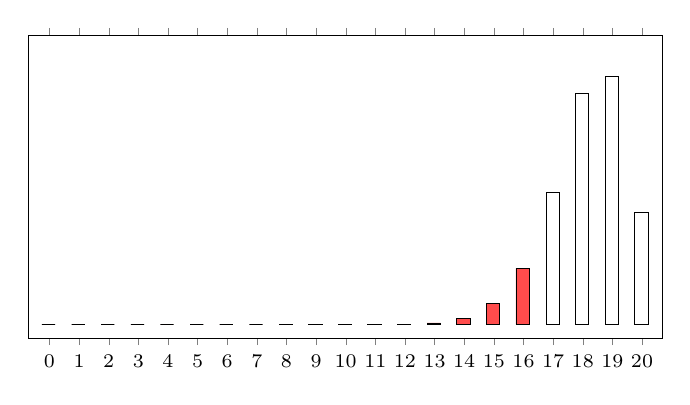
\begin{tikzpicture}[scale = 0.6]
\begin{axis}[
    ybar,
    bar width=8pt,
    enlargelimits=0.05,
    xtick={0,...,20},
    ytick = \empty,
    tick label style={font=\scriptsize, scale = 1/0.6},
    ymin=0,
    ymax=0.3,
    legend style={at={(0.5,-0.15)}, anchor=north, legend columns=-1},
    width=15cm,
    height=8cm
]

% Highlighted bars: X <= 16
\addplot[
    ybar,
    fill=red!70,
    draw=black
] coordinates {
    (0.25, 1.024e-19)
    (1.25, 2.048e-18)
    (2.25, 1.943e-16)
    (3.25, 1.166e-14)
    (4.25, 4.872e-13)
    (5.25, 1.4606e-11)
    (6.25, 3.2475e-10)
    (7.25, 5.6315e-09)
    (8.25, 7.6149e-08)
    (9.25, 8.4604e-07)
    (10.25, 7.4864e-06)
    (11.25, 5.4512e-05)
    (12.25, 0.0003269)
    (13.25, 0.0016275)
    (14.25, 0.0067456)
    (15.25, 0.0226)
    (16.25, 0.0609)
};

% Non-highlighted bars: X > 16
\addplot[
    ybar,
    fill=gray!0,
    draw=black
] coordinates {
    (16.7, 0.1432)
    (17.7, 0.2511)
    (18.7, 0.2702)
    (19.7, 0.1216)
};

\end{axis}
\end{tikzpicture}
\end{center}

%Pictures of binomial dist with tail shaded

%If the number of successful shots is small enough that someone who makes 90\% of their free throws should almost always exceed it, we have strong evidence against Charles' claim.

The value of $P(X \leq 16)$ measures the cumulative probability in the tail, shown above in red, which tells us how far into the tail we've gone. To assess the strength of our experimental evidence, instead of using the probability of observing \emph{precisely} the evidence we have seen, we use the probability of observing evidence \emph{at least as strong} as the evidence we've seen.

\begin{note}
In the earlier tea tasting example, we also computed the probability of observing evidence \emph{at least as strong} as what we observed. It happened that in this case, Alice's selection was perfect, so she produced the strongest possible evidence she can taste the difference. If she had only selected four of the five cups that were poured milk first, and also made one incorrect selection, we would have computed the probability of selecting four or more correct cups by chance.
\end{note}

\subsection*{Statistical Hypotheses}

In the language of statistical tests, each test has a \newterm{null hypothesis}\index{Null Hypothesis}, denoted $H_0$, and an \newterm{alternative hypothesis}\index{Alternative Hypothesis}, denoted $H_a$.

In our tea tasting example, the null hypothesis, $H_0$, is that Alice cannot tell the difference between the two methods of pouring tea by tasting, and $H_a$ is that she can, and moreover, can even determine which of the two methods was used.

In our basketball example, the null hypothesis, $H_0$, is that Charles is a 90\% free throw shooter, and $H_a$ is that his free throw percentage is lower. Note that in this context, we interpret Charles' claim as a boast that he is a very good free throw shooter. This means if Charles were to make twenty out of twenty free throws, we would interpret this as evidence for his claim, not against it. 

The null hypothesis is often a statement that a certain procedure has no effect, or that a parameter is equal to a certain claimed value. In a statistical test, we do an experiment which may produce evidence for the alternative hypothesis, and decrease our confidence that the null hypothesis is correct. If this evidence is strong enough, we reject the null hypothesis, and conclude the alternative. The strength of the evidence is quantified as follows.

\begin{definition}
The \newterm{P-value}\index{P-value} in a test of $H_0$ against $H_a$ is the probability of observing evidence for $H_a$ which is at least as strong as the evidence we saw in the experiment, given that $H_0$ is true.
\end{definition}

How small does this probability need to be to convince us the null hypothesis is no longer believable in light of the evidence? This can depend on the context, but the most typical value used is 0.05, or 5\%, and this cutoff is referred to as the \newterm{significance level}\index{Significance Level} of the test. We'll discuss the details of this choice later, in Section \ref{TestPower}.

\begin{example}\label{MagicCoinEx}
You meet someone who claims to be a wizard. He says he can cast a spell that will cause a fair coin to land on heads more often than tails. You pull a coin from your pocket and ask him to cast the spell. After he does, you flip the coin thirty times, resulting in eighteen heads and twelve tails. Is this enough evidence, at the 5\% significance level, to conclude his spell actually works?

Here the null hypothesis is that the spell had no effect, so the coin is still fair. The alternative is that the probability of heads has increased. If we let $p$ denote the probability of heads after the spell has been cast, then we can abbreviate the hypotheses as $H_0: p = \frac{1}{2}$ and $H_a: p > \frac{1}{2}$. 

Under the null hypothesis, the number of heads we observe in thirty flips is $X \sim \Binomial(30,0.5)$. We observed a sample with eighteen heads, so the $P$-value for the test is $P(X \geq 18) \approx 0.181$, which was computed by summing up the binomial probabilities $P(X = 18) + P(X = 19) + \,\cdots\, + P(X = 30)$.

\begin{center}
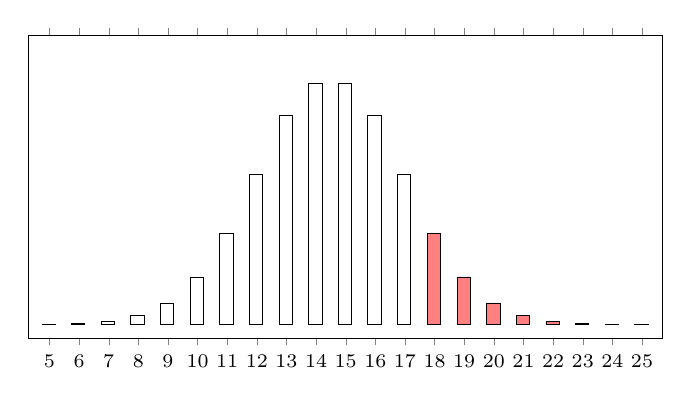
\begin{tikzpicture}[scale = 0.6]
\begin{axis}[
    tick label style={font=\scriptsize, scale = 1/0.6},
    ybar,
    bar width=8pt,
    enlargelimits=0.05,
    xtick={5,...,25},
    ytick = \empty,
    ymin=0,
    ymax=0.165,
    legend style={at={(0.5,-0.15)}, anchor=north, legend columns=-1},
    width=15cm,
    height=8cm
]

% Highlighted bars: X <= 16
\addplot[
    ybar,
    fill=gray!0,
    draw=black
] coordinates {
(5.25, 0.000137090682983398)
(6.25, 0.000549554824829102)
(7.25, 0.0018312931060791)
(8.25, 0.00514936447143555)
(9.25, 0.0128737688064575)
(10.25, 0.0283775329589844)
(11.25, 0.0542540550231934)
(12.25, 0.08966064453125)
(13.25, 0.12516975402832)
(14.25, 0.144524574279785)
(15.25, 0.144524574279785)
(16.25, 0.12516975402832)
(17.25, 0.08966064453125)
};

% Non-highlighted bars: X > 16
\addplot[
    ybar,
    fill=red!50,
    draw=black
] coordinates {
(17.7, 0.0542540550231934)
(18.7, 0.0283775329589844)
(19.7, 0.0128737688064575)
(20.7, 0.00514936447143555)
(21.7, 0.0018312931060791)
(22.7, 0.000549554824829102)
(23.7, 0.000137090682983398)
(24.7, 2.64549255371094e-05)
};

\end{axis}
\end{tikzpicture}
\end{center}

Since $P >0.05$, we conclude that we have not seen enough evidence to reject the null hypothesis at the 5\% significance level. In other words, the coin has not shown sufficient bias in this sample of flips for us to believe the spell actually had an effect.
\end{example}

In summary, a hypothesis test to assess the strength of experimental evidence for an alternative hypothesis $H_a$ against a null hypothesis $H_0$, at a given significance level, proceeds as follows:
\begin{enumerate}[label=\Roman*.]
\item State the null hypothesis $H_0$ and the alternative hypothesis $H_a$.
\item Under the assumption that $H_0$ is true, compute the probability of observing evidence for $H_a$ which is at least as strong as the evidence observed in the experiment (the $P$-value of the test).
\item If the $P$-value is below the significance level, we have seen sufficient evidence to reject $H_0$ and conclude $H_a$, if not, our experiment did not produce strong enough evidence to reject $H_0$.
\end{enumerate}

\begin{keypoint}
If we observe strong enough evidence for the alternative, we \emph{reject} the null hypothesis. If not, then we \emph{do not reject} the null hypothesis. We never conclude the null hypothesis is true.
\end{keypoint}

This asymmetry is important to note. In the basketball example above, there is no way to convince ourselves that Charles' free throw shooting percentage is \emph{exactly} 90\% by using experimental data. We could produce a confidence interval for his shooting percentage, but no matter how small the interval, the exact value 0.9 is one of infinitely many other possible values in the interval.

One useful analogue is to imagine that someone in the room claims the temperature is $21.7^\circ$\,C, but the only thermometer available could be off by up to $2^\circ$\,C. If the thermometer reads $22.3^\circ$\,C (or even if it reads $21.7^\circ$\,C), you can't tell whether the claim is true or false, but if the thermometer reads $25.2^\circ$\,C, you know the claim is false.

\section{Hypothesis Test on a Population Mean}\index{Hypothesis Test! on a Mean}

In an old textbook, it's written that during the month of July, the mean daily high in Montreal is $26.2^{\circ}$\,C, with a standard deviation of $3.2^{\circ}$\,C. You wonder if this could still be true, so you take a sample of fifty days in July from the last decade, look up the daily high in Montreal for each, and find the the mean daily high in your sample is $27.3^{\circ}$\,C. Is this enough evidence to conclude the mean daily high in July over the last decade is above $26.2^{\circ}$\,C, at the 5\% significance level?

To answer this question, we can test the null hypothesis that the mean daily high last decade is still $26.2^{\circ}$\,C against the alternative that it's higher. These are both claims about the mean daily high for all days in July over the last decade, which is our population in this scenario. Therefore, letting $\mu$ denote the mean daily high for all days in July over the last decade, we can write the hypotheses as
$$H_0: \mu = 26.2 \text{\ \ and \ \ }H_a: \mu > 26.2.$$

Next, note that our sample mean, $\littlexbar = 27.3$, can be regarded as a realization of a Gaussian random variable. Why? We can appeal to the central limit theorem because our sample is a random sample and sufficiently large. Therefore, we can compute the probability of observing a value of $\xbar$ at least as high as the one in our sample under the null hypothesis that the mean temperature has not changed (the $P$-value of the test) by standardizing our sample mean
$$z = \frac{\littlexbar - \mu_{0}}{\frac{\sigma}{\sqrt{n}}}$$
and then using the $Z$-table. Since the test is done using the mean of a single sample, and the $P$-value is computed using the $Z$-table, this hypothesis test is known as the \newterm{one sample Z-test}.

\begin{remark}
In order the compute the test statistic $Z$, we'll need to know the population standard deviation $\sigma$. We would essentially never have this information in practice. In this example, we'll take $\sigma = 3.2$, which is not strictly correct (even if we believe the values in the old textbook were computed from a complete set of data at the time it was published, the standard deviation of daily highs in July has likely changed since then). First let's see how the test works, then we'll deal with this issue.
\end{remark}

\begin{example}
In an old textbook, it's written that during the month of July, the mean daily high in Montreal is $26.2^{\circ}$\,C, with a standard deviation of $3.2^{\circ}$\,C. You wonder if this could still be true, so you take a sample of fifty days in July from the last decade, look up the daily high in Montreal for each, and find the the mean daily high in your sample is $27.3^{\circ}$\,C. Is this enough evidence to conclude the mean daily high in July over the last decade is above $26.2^{\circ}$\,C, at the 5\% significance level?

\begin{enumerate}[label=\textnormal{\Roman*}.]
\item $H_0: \mu = 26.2$, $H_a: \mu > 26.2$.

\item Our test statistic is $z = \frac{\littlexbar - \mu_{0}}{\frac{\sigma}{\sqrt{n}}} = \frac{27.3 - 26.2}{\frac{3.2}{\sqrt{50}}} = 2.43$.

The P-value is the probability of obtaining a sample whose test statistic is at least as large as the one we observed, that is, the area under the standard normal distribution to the right of $2.43$.
\begin{center}
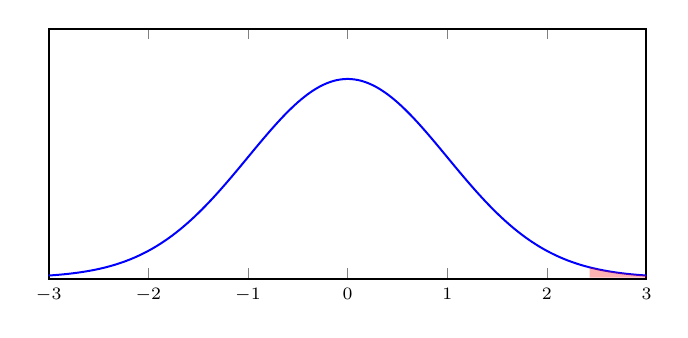
\begin{tikzpicture}[scale = 0.9]
  \begin{axis}[
  	  scale only axis,
      unit vector ratio=1 5 1,
      ymin=-0.0025,
      ymax=0.5,
      xmin=-3,
      xmax=3,
      tick label style={font=\scriptsize, scale = 1/1},
      xtick={-3,-2,-1,0,1,2,3},
      ytick=\empty,
      legend pos=north east,
      domain=-3:3,
      samples=200,
      thick
    ]

    \addplot[blue]  {(1/2.50663)*exp(-x*x/2)};
    
    \addplot[blue, opacity=0, fill=red, fill opacity=0.3, domain=2.43:3] 
      {(1/2.50663)*exp(-x*x/2)} \closedcycle;

  \end{axis}
\end{tikzpicture}
\end{center}
Thus, the P-value is $P(Z \geq 2.43) = 1 - P(Z \leq 2.43) = 1 - 0.9925 = 0.0075$.

\item Since $P < 0.05$, we have seen sufficient evidence to conclude that the mean daily high in July over the last decade in Montreal is above $26.2^{\circ}$\,C, at the 5\% significance level.
\end{enumerate}
\end{example}

\begin{example}
A bicycle components manufacturer claims the mean diameter of crank axles they produce is $24.98$\,mm with a standard deviation of $0.05$\,mm. A random sample of thirty-eight axles were measured very accurately, the mean diameter was found to be $24.968$\,mm. Is this enough evidence to conclude the mean diameters of axles the manufacturer is producing is not $24.98\,mm$, at the 5\% significance level?

Note that in this example, we have a \newterm{two-sided alternative hypothesis}. We're looking for evidence the mean axle diameter \textbf{is not} $24.98$\,mm. Contrast this with the last example, where we had a \newterm{one-sided alternative hypothesis}. We were looking for evidence the mean temperature was \textbf{above} $26.2^{\circ}$\,C.

\begin{keypoint}
The alternative hypothesis is chosen based on what the researchers want to be able to conclude from the test. Is the goal of the experiment to show that the population mean is higher than a certain claimed value, lower than a certain claimed value, or not equal to that value?
\end{keypoint}

\begin{enumerate}[label=\textnormal{\Roman*}.]
\item $H_0: \mu = 24.98$, $H_a: \mu \neq 24.98$.

\item Our test statistic is $z = \frac{\littlexbar - \mu_{0}}{\frac{\sigma}{\sqrt{n}}} = \frac{24.968 - 24.98}{\frac{0.05}{\sqrt{38}}} = -1.48$.

The P-value is the probability of obtaining a sample whose test statistic is at least as far from zero as the one we observed, that is, the area under the standard normal distribution the left of $-1.48$ and to the right of $1.48$.
\begin{center}
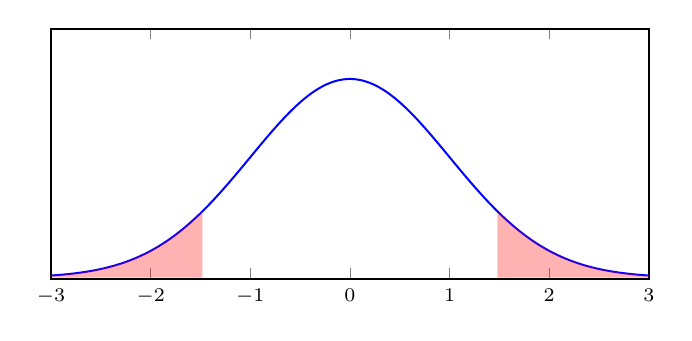
\begin{tikzpicture}[scale = 0.9]
  \begin{axis}[
  	  scale only axis,
      unit vector ratio=1 5 1,
      ymin=-0.0025,
      ymax=0.5,
      xmin=-3,
      xmax=3,
      tick label style={font=\scriptsize, scale = 1/0.9},
      xtick={-3,-2,-1,0,1,2,3},
      ytick=\empty,
      legend pos=north east,
      domain=-3:3,
      samples=200,
      thick
    ]

    \addplot[blue]  {(1/2.50663)*exp(-x*x/2)};
    
    \addplot[blue, opacity=0, fill=red, fill opacity=0.3, domain=1.48:3] 
      {(1/2.50663)*exp(-x*x/2)} \closedcycle;
      
      \addplot[blue, opacity=0, fill=red, fill opacity=0.3, domain=-3:-1.48] 
      {(1/2.50663)*exp(-x*x/2)} \closedcycle;

  \end{axis}
\end{tikzpicture}
\end{center}
Thus, the P-value is $P(Z \geq 1.48) + P(Z \leq -1.48) = 2\,P(Z \leq -1.48) = 0.1388$.

\item Since $P > 0.05$, we have not seen sufficient evidence to conclude the mean diameters of axles the manufacturer is producing is different from $24.98\,mm$, at the 5\% significance level
\end{enumerate}
\end{example}

Note that in the last two examples, we tested claims about the population mean $\mu$, and in our test, used the population standard deviation $\sigma$ provided by the same authority that gave us the value of $\mu$ we had doubts about (in the first example, a textbook, and in the second, a bicycle components manufacturer), which seems problematic. Indeed, the conclusion of the test is only properly justified if the value of $\sigma$ used in the test is the true population standard deviation, which is essentially always unknown in practice.

\subsection*{What if we don't know $\sigma$?}

We've dealt with this problem when constructing confidence intervals, and fortunately, the same approach extends to hypothesis testing. Using the sample standard deviation $s$ in place of the parameter $\sigma$, we can calculate the test statistic
$$t = \frac{\littlexbar - \mu_{0}}{\frac{s}{\sqrt{n}}}.$$

The hypothesis test will proceed in the same way, but to calculate the $P$-value we'll need to use the $T$-distribution with $n-1$ degrees of freedom in place of the standard normal distribution. Since the test is done using data from a single sample, and the $P$-value is computed using the $T$-table, this hypothesis test is known as the \newterm{one sample T-test}.

\begin{remark}
Notice that the $T$-distribution is used to account for the additional variability introduced by using the sample standard deviation $s$ as an estimate for the population standard deviation $\sigma$. This is done when constructing confidence intervals and also when performing hypothesis tests.
\end{remark}

\begin{example}
An insurance company claims that customers who switch to their insurance policies save an average of \$15 on their monthly car insurance payment. Monthly payments in a random sample of 12 customers that switched to this company are given below, before and after the switch, each column representing a single customer.
\begin{center}\begin{tabular}{rcccccccccccccc}
Pre-Switch & 70 & 115 & 96 & 84 & 97 & 72 & 90 & 83 & 77 & 121 & 101 & 93 \\
Post-Switch & 67 & 92 & 82 & 86 & 74 & 65 & 75 & 74 & 71 & 89 & 91 & 78 \\
\end{tabular}\end{center}

Is this enough evidence to conclude that, on average, customers who switch do not save as much as the company claims, at the 5\% significance level?

To evaluate a claim about savings, first we'll need to compute the savings for each customer in the sample. Doing so gives the results below. The mean amount saved in the sample is $\littlexbar = 12.92$ with a standard deviation of $s = 9.56$. The null hypothesis of the test is that the mean savings is \$15, and the alternative is that it's smaller.
\begin{center}\begin{tabular}{rcccccccccccccc}
Pre-Switch & 70 & 115 & 96 & 84 & 97 & 72 & 90 & 83 & 77 & 121 & 101 & 93 \\
Post-Switch & 67 & 92 & 82 & 86 & 74 & 65 & 75 & 74 & 71 & 89 & 91 & 78 \\
Savings & 3 & 23 & 14 & -2 & 23 & 7 & 15 & 9 & 6 & 32 & 10 & 15 \\
\end{tabular}\end{center}

\begin{enumerate}[label=\textnormal{\Roman*}.]
\item $H_0: \mu = 15$, $H_a: \mu < 15$.

\item Our test statistic is $t = \frac{\littlexbar - \mu_{0}}{\frac{s}{\sqrt{n}}} = \frac{12.92 - 15}{\frac{9.56}{\sqrt{12}}} = -0.75$.

The P-value is the probability of obtaining a sample whose test statistic is at least as small as the one we observed, that is, the area to the left of $-0.75$ under the T-distribution with 11 degrees of freedom.
\begin{center}
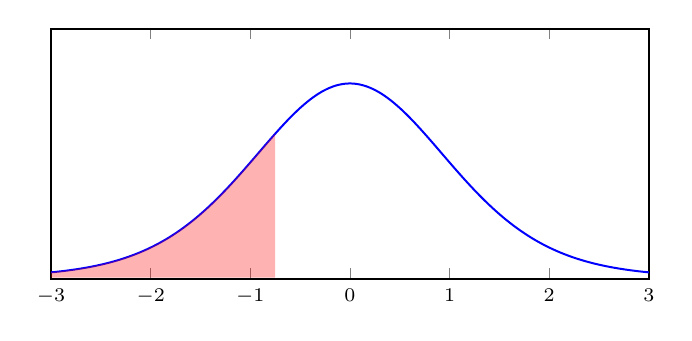
\begin{tikzpicture}[scale = 0.9]
  \begin{axis}[
  	  scale only axis,
      unit vector ratio=1 5 1,
      ymin=-0.0025,
      ymax=0.5,
      xmin=-3,
      xmax=3,
      tick label style={font=\scriptsize, scale = 1/0.9},
      xtick={-3,-2,-1,0,1,2,3},
      ytick=\empty,
      legend pos=north east,
      domain=-3:3,
      samples=200,
      thick
    ]

    \addplot[blue]  {0.39*(1+(x*x)/11)^(-6)};
      
      \addplot[blue, opacity=0, fill=red, fill opacity=0.3, domain=-3:-0.75] 
      {0.39*(1+(x*x)/11)^(-6)} \closedcycle;

  \end{axis}
\end{tikzpicture}
\end{center}
Consulting a table of values for the T-distribution, we can find the critical value which produces a tail area of 5\% is $-1.796$. Therefore, the P-value in our test is (much) larger than 5\%. Using a computer to explicitly compute the area gives $P = 0.234$.

\item Since $P > 0.05$, we have not seen sufficient evidence to conclude the mean monthly savings is less than \$15, at the 5\% significance level.
\end{enumerate}
\end{example}

\begin{warning}
The hypothesis test above is not properly justified! The sample consisted of only twelve individuals. Moreover, we are in a context where we have no reason to believe the population distribution under consideration (the distribution of the amount saved by switching) is Gaussian.
\end{warning}

It happened that the conclusion of the test was that there is not enough evidence in our sample to conclude the claim is false, which was the status quo before we did the test, so there's no harm done. But it's important to recognize that the $P$-value, which determines the conclusion of the test, is only an accurate assessment of the strength of evidence in our sample when the approximation given by the central limit theorem is accurate. In situations where this is not the case, one should simply refuse to use the methods of this section (and the next), and appeal to other methods instead.

\section{Hypothesis Test on a Population Proportion}\index{Hypothesis Test! on a Proportion}

In Example \ref{MagicCoinEx}, we tested whether a coin which had a magic spell cast on it had become biased towards heads, which was the supposed effect of the spell, by flipping it thirty times. In the sample of thirty flips, eighteen were heads. Letting $p$ denote the actual proportion of heads for this coin, our hypotheses were $H_0: p = \frac{1}{2}$ (the coin is fair) and $H_a: p > \frac{1}{2}$ (the coin is biased towards heads). 

We calculated the $P$-value directly from the binomial distribution, but calculating a tail probability of a binomially distributed random variable is tedious. Let's do the same test, but this time we'll use the central limit theorem to make the $P$-value calculation much more routine.

For a Bernoulli distributed random variable (which counts the number of heads in a single flip of a coin), the mean is $\mu = p$ and the standard deviation is $\sigma = \sqrt{p(1-p)}$. This means the null hypothesis $H_0: p = \frac{1}{2}$ is not just a claim about the population mean $\mu$, it's also a claim about the population standard deviation $\sigma$.

\begin{keypoint}
If in fact $p = \frac{1}{2}$, we are sampling from a population distribution with $\mu = \frac{1}{2}$ and $\sigma = \sqrt{\frac{1}{2}(1-\frac{1}{2})}$.
\end{keypoint}

The $P$-value is the probability of observing evidence at least as strong as what was observed in our sample, \emph{assuming $H_0$ is true}, so for the purposes of calculating the $P$-value, the population standard deviation $\sigma$ is known, and we can use the $Z$-test, exactly as in the last section. 

If we let $p_0$ denote the claimed proportion in the null hypothesis ($\frac{1}{2}$ in our example), $\widehat{p}$ denote the proportion observed in our sample ($\frac{18}{30}$ in our example), and make the replacements $\mu = p_0$ and $\sigma = \sqrt{p_0(1-p_0)}$, our test statistic becomes

$$z = \frac{\widehat{p} - p_0}{\sqrt{\frac{p_0(1-p_0)}{n}}}.$$

\begin{example}
You meet someone who claims to be a wizard. He says he can cast a spell that will cause a fair coin to land on heads more often than tails. You pull a coin from your pocket and ask him to cast the spell. After he does, you flip the coin thirty times, resulting in eighteen heads and twelve tails. Is this enough evidence, at the 5\% significance level, to conclude his spell actually works?

\begin{enumerate}[label=\textnormal{\Roman*}.]
\item $H_0: p = \frac{1}{2}$, $H_a: p > \frac{1}{2}$.

\item Our test statistic is $z = \frac{\widehat{p} - p_0}{\sqrt{\frac{p_0(1-p_0)}{n}}} = \frac{\frac{18}{30} - \frac{1}{2}}{\sqrt{\frac{\frac{1}{2}(1-\frac{1}{2})}{30}}} = 1.10$.

The P-value is the probability of obtaining a sample whose test statistic is at least as large as the one we observed, that is, the area under the standard normal distribution to the right of $1.10$.
\begin{center}
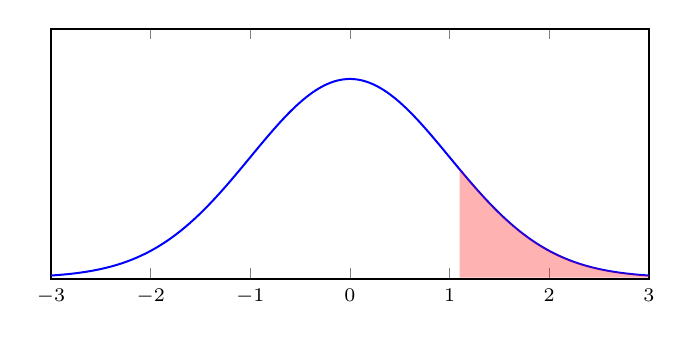
\begin{tikzpicture}[scale = 0.9]
  \begin{axis}[
  	  scale only axis,
      unit vector ratio=1 5 1,
      ymin=-0.0025,
      ymax=0.5,
      xmin=-3,
      xmax=3,
      tick label style={font=\scriptsize, scale = 1/0.9},
      xtick={-3,-2,-1,0,1,2,3},
      ytick=\empty,
      legend pos=north east,
      domain=-3:3,
      samples=200,
      thick
    ]

    \addplot[blue]  {(1/2.50663)*exp(-x*x/2)};
    
    \addplot[blue, opacity=0, fill=red, fill opacity=0.3, domain=1.10:3] 
      {(1/2.50663)*exp(-x*x/2)} \closedcycle;

  \end{axis}
\end{tikzpicture}
\end{center}
Thus, the P-value is $P(Z \geq 1.10) = 1 - P(Z \leq 1.10) = 1 - 0.8643 = 0.1357$.

\item Since $P > 0.05$, we have not seen sufficient evidence to conclude that the coin is biased towards heads, at the 5\% significance level.
\end{enumerate}
\end{example}

Note that even though the conclusion is the same as it was in Example \ref{MagicCoinEx}, the $P$-value is not. The majority of the discrepancy is due to the continuous approximation given by the central limit theorem. In Example \ref{MagicCoinEx}, the $P$-value included the probability exactly 18 heads are observed, but not the probability 19 heads are observed. To mimic this in our continuous approximation, we can use $\widehat{p} = \frac{18.5}{30}$ instead of $\widehat{p} = \frac{18}{30}$ in our test, to have an even split between the two borderline cases. This is known as a continuity correction. We won't cover this in the course, but it's a good exercise to run through the test again with this change, and see that the $P$-value comes out very close to the value we obtained by working directly with the binomial distribution. 

As the sample size increases, the continuity correction will have a smaller and smaller effect on the $P$-value of the test, so as long as the sample size is large enough, the discrepancy between the $P$-values will be insignificant.

\begin{example}
A botanist estimates that $73$\% of the mature trees in a forest are maples. In a random sample of 200 mature trees, 161 of them were maples. Is this enough evidence to conclude the botanist's estimate is not correct, at the 5\% significance level?

We're assessing whether our sample data is enough to convince us the botanist's estimate of $73$\% is incorrect, so the test will use a two-sided alternative. The botanist's estimate could be incorrect by being either too low or too high.

\begin{enumerate}[label=\textnormal{\Roman*}.]
\item $H_0: p = 0.73$, $H_a: p \neq 0.73$.

\item Our test statistic is $z = \frac{\widehat{p} - p_0}{\sqrt{\frac{p_0(1-p_0)}{n}}} = \frac{\frac{161}{200} - 0.73}{\sqrt{\frac{0.73(1-0.73)}{200}}} = 2.39$.

The P-value is the probability of obtaining a sample whose test statistic is at least as far from zero as the one we observed, that is, the area under the standard normal distribution to the left of $-2.39$ and to the right of $2.39$.
\begin{center}
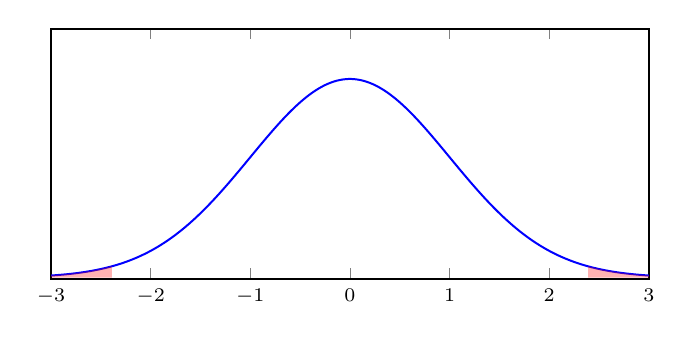
\begin{tikzpicture}[scale = 0.9]
  \begin{axis}[
  	  scale only axis,
      unit vector ratio=1 5 1,
      ymin=-0.0025,
      ymax=0.5,
      xmin=-3,
      xmax=3,
      tick label style={font=\scriptsize, scale = 1/0.9},
      xtick={-3,-2,-1,0,1,2,3},
      ytick=\empty,
      legend pos=north east,
      domain=-3:3,
      samples=200,
      thick
    ]

    \addplot[blue]  {(1/2.50663)*exp(-x*x/2)};
    
    \addplot[blue, opacity=0, fill=red, fill opacity=0.3, domain=2.39:3] 
      {(1/2.50663)*exp(-x*x/2)} \closedcycle;
      
      \addplot[blue, opacity=0, fill=red, fill opacity=0.3, domain=-3:-2.39] 
      {(1/2.50663)*exp(-x*x/2)} \closedcycle;

  \end{axis}
\end{tikzpicture}
\end{center}
Thus, the P-value is $P(Z \geq 2.39) + P(Z \leq -2.39) = 2\,P(Z \leq -2.39) = 0.0164$.

\item Since $P < 0.05$, we have seen sufficient evidence to conclude the botanist's estimate of $73$\% maples is incorrect, at the 5\% significance level.
\end{enumerate}
\end{example}

\begin{keypoint}
Regardless of whether we're doing a hypothesis test on a mean or proportion, and in the former case, regardless of whether we are given the population standard deviation $\sigma$ or not, we follow the same three-step procedure. It's just the test statistic that changes.
\begin{center}
\begin{tabular}{c|c|c}
Mean with $\sigma$ & Mean with $s$ & Proportion  \\ \hline & & \\[-2ex]
$z = \frac{\littlexbar - \mu_{0}}{\frac{\sigma}{\sqrt{n}}}$ & $t = \frac{\littlexbar - \mu_{0}}{\frac{s}{\sqrt{n}}}$ & $z = \frac{\widehat{p} - p_0}{\sqrt{\frac{p_0(1-p_0)}{n}}}$
\end{tabular}
\end{center}
Note that the name of the test statistic indicates which distribution to use when computing the $P$-value of the test, and in each case, the test can be done with a one-sided or two-sided alternative hypothesis.
\end{keypoint}

\section{Significance, Confidence, \& Power}\label{TestPower}

Each hypothesis test ends with a decision to either reject the null hypothesis, and conclude the alternative is correct, or refuse to reject the null hypothesis because we have not observed strong enough evidence against it in our sample.

This means there are only two ways to come to the \emph{incorrect} conclusion, either by rejecting the null hypothesis when, in fact, it's true, or by not rejecting the null hypothesis when, in fact, the alternative is true. These are unfortunately known by the uninspiring names \newterm{Type I error}\index{Type I Error} and \newterm{Type II error}\index{Type II Error}.
\begin{center}
\begin{tabular}{|c|c|c|}
\hline
\textbf{Decision} & \textbf{$H_0$ is True} & \textbf{$H_a$ is True} \\
\hline
Do not reject $H_0$ & Correct & Type II Error \\
\hline
Reject $H_0$ & Type I Error & Correct \\
\hline
\end{tabular}
\end{center}

\begin{remark}
A useful analogy here is a jury trial. The defendant is only deemed guilty if the there's sufficient evidence, so $H_0$ is innocence and $H_a$ is guilt. In this context, convicting an innocent defendant is a Type I error, and acquitting a guilty defendant is a Type II error.
\end{remark}

To understand how these occur, consider a one-sample $Z$-test of $H_0: \mu = \mu_0$ against $H_a: \mu > \mu_0$, done at the 5\% significance level, as usual.

We've seen that the distribution of the sample mean $\xbar$ is centred at the population mean $\mu$, and if the hypotheses of the central limit theorem hold, is approximately Gaussian. In the figures below, we'll draw this distribution in blue. The null hypothesis, which may or may not be true, claims the population mean is $\mu_0$.

\begin{center}
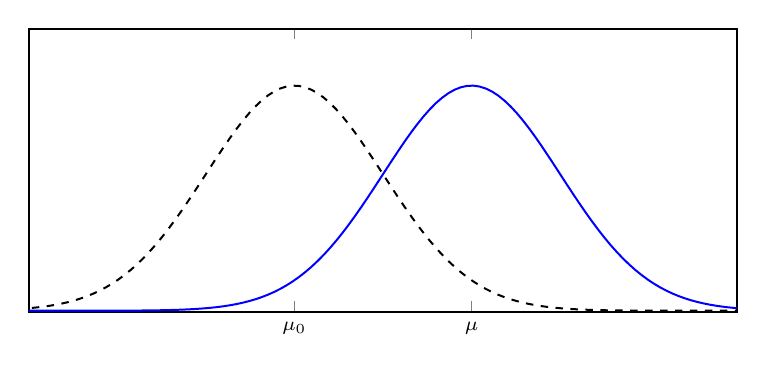
\begin{tikzpicture}[scale = 0.9]
  \begin{axis}[
  	  scale only axis,
      width=10cm,
      height=4cm,
      ymin=-0.0025,
      ymax=0.5,
      xmin=-4,
      xmax=4,
      tick label style={font=\scriptsize, scale = 1/0.9},
      xtick={-1,1},
      xticklabels={$\mu_0$,$\mu$},
      ytick=\empty,
      legend pos=north east,
      domain=-7:7,
      samples=200,
      thick
    ]

    \addplot[black, dashed]  {(1/2.50663)*exp(-(x+1)*(x+1)/2)};
    %\addplot[black, thin] (-1,0) -- (-1,1/2.50663);
   
    \addplot[blue]  {(1/2.50663)*exp(-(x-1)*(x-1)/2)};

  \end{axis}
\end{tikzpicture}
\end{center}

We'll call these two distributions the \newterm{true distribution}\index{True Distribution} of $\xbar$ (centred at the true mean $\mu$), and the \newterm{null distribution}\index{Null Distribution} of $\xbar$ (centred at at the hypothesized value $\mu_0$) respectively. Note that when we calculate the test statistic, we use the hypothesized mean $\mu_0$.

Now if the null hypothesis is, in fact, true, then the two distributions are identical, and the correct decision is to not reject $H_0$. We'll incorrectly reject $H_0$ (a Type I error) when the area to the right of the test statistic (the $P$-value) is under $5\%$, which happens when our sample is among the $5\%$ highest samples, in terms of the sample mean.

\begin{center}
\begin{tikzpicture}[scale = 0.9]
  \begin{axis}[
  	  scale only axis,
      width=8cm,
      height=4cm,
      ymin=-0.0025,
      ymax=0.5,
      xmin=-3.5,
      xmax=3.5,
      tick label style={font=\scriptsize, scale = 1/0.9},
      xtick={0},
      xticklabels={$\mu_0 = \mu$},
      ytick=\empty,
      legend pos=north east,
      domain=-7:7,
      samples=200,
      thick
    ]
   
    \addplot[blue]  {(1/2.50663)*exp(-(x)*(x)/2)};
    
    \addplot[blue, opacity=0, fill=red, fill opacity=0.3, domain=1.96:3.5] 
      {(1/2.50663)*exp(-x*x/2)} \closedcycle;
      
      \addplot[blue, opacity=0, fill=green, fill opacity=0.3, domain=-3.5:1.96] 
      {(1/2.50663)*exp(-x*x/2)} \closedcycle;
      
      \addplot[black, dashed]  {(1/2.50663)*exp(-(x)*(x)/2)};
      
      \node at (axis cs:0,0.165) {$1-\alpha$};
    
     \addplot[blue, opacity=0, fill=none, fill opacity=1, domain=1.96:4, postaction={pattern=north east lines}] 
      {(1/2.50663)*exp(-(x)*(x)/2)} \closedcycle;

  \end{axis}
\end{tikzpicture}
\end{center}

Thus, when we choose the significance level of the test, we're setting the probability of a Type I error. Why not always take a very small significance level then, since making a Type I error is something we would ideally never do?

The problem comes when the null hypothesis is false. If the population mean $\mu$ is higher than $\mu_0$, the correct decision is to reject $H_0$. In this situation, a Type II error will occur if the $P$-value is above $5\%$. When we select a random sample, its mean is drawn from the true distribution of $\xbar$ (the blue distribution), then we take that realization $\littlexbar$ and compute the $P$-value using the null distribution of $\xbar$ (the dashed black distribution). 

The green area below is the probability of correctly rejecting $H_0$ (obtaining a sample whose test statistic is far enough into the tail of the null distribution to have $P < 0.05$), and the red area is the probability of not rejecting $H_0$ (obtaining a sample with $P > 0.05$).

\begin{center}
\begin{tikzpicture}[scale = 0.9]
  \begin{axis}[
  	  scale only axis,
      width=10cm,
      height=4cm,
      ymin=-0.0025,
      ymax=0.5,
      xmin=-2.5,
      xmax=5.5,
      tick label style={font=\scriptsize, scale = 1/0.9},
      xtick={0,3},
      xticklabels={$\mu_0$,$\mu$},
      ytick=\empty,
      legend pos=north east,
      domain=-2.5:5.5,
      samples=200,
      thick
    ]
    
    \addplot[blue, opacity=0, fill=green, fill opacity=0.3, domain=1.96:5.5] 
      {(1/2.50663)*exp(-(x-3)*(x-3)/2)} \closedcycle;
      
      \addplot[blue, opacity=0, fill=red, fill opacity=0.3, domain=-3:1.96] 
      {(1/2.50663)*exp(-(x-3)*(x-3)/2)} \closedcycle;

    \addplot[black, dashed]  {(1/2.50663)*exp(-(x)*(x)/2)};
    %\addplot[black, thin] (-1,0) -- (-1,1/2.50663);
   
    \addplot[blue]  {(1/2.50663)*exp(-(x-3)*(x-3)/2)};
    
    \node at (axis cs:3,0.165) {$1-\beta$};
    
    \addplot[blue, opacity=0, fill=none, fill opacity=1, domain=1.96:4, postaction={pattern=north east lines}] 
      {(1/2.50663)*exp(-(x)*(x)/2)} \closedcycle;
    
  \end{axis}
\end{tikzpicture}
\end{center}

The probability of not rejecting $H_0$ when it's true is the \newterm{confidence}\index{Confidence Level! of a Hypothesis Test} level of the test, denoted $1-\alpha$, and the probability of rejecting $H_0$ when it's false is called the \newterm{power}\index{Power! of a Hypothesis Test} of the test, denoted $1- \beta$. As we increase the confidence level (that is, decrease the significance level) of the test, the Type I error rate ($\alpha$) shrinks, but the Type II error rate ($\beta$) grows.
\begin{center}
\begin{tabular}{|c|c|c|}
\hline
\textbf{Decision} & \textbf{$H_0$ is True} & \textbf{$H_a$ is True} \\
\hline
Do not reject $H_0$ & $1-\alpha$ & $\beta$ \\
\hline
Reject $H_0$ & $\alpha$ & $1-\beta$ \\
\hline
\end{tabular}
\end{center}

\begin{keypoint}
There is a tradeoff between confidence and power. A test done at the 1\% significance level has a higher confidence level, but lower power, than a test done at the 5\% significance level.
\end{keypoint}

\subsection*{Effect Size, Sample Size, and Significance}

The difference between the true mean $\mu$ and the hypothesized mean $\mu_0$ is often referred to as the \newterm{effect size}\index{Effect Size}. Consider for example a new cold medication on the market. If those who have a cold and take no medication have symptoms for a mean of 5.7 days, and those who have a cold and take the new medication have symptoms for a mean of 5.2 days, one could say the effect of the medication was to decrease the mean symptom length by 0.5 days.

A hypothesis test is an assessment of the strength of evidence for an effect (potentially in a certain direction depending on the alternative hypothesis chosen) in sample data, and the power of the test, $\beta$, is the probability of detecting an effect when an effect actually exists. When we reject $H_0$ and conclude that we've seen sufficient evidence for an effect, it's common to say that our study or experiment has produced a \newterm{statistically significant}\index{Statistical Significance} result.

\begin{remark}
Notice that as the effect size increases, and $\mu$ moves farther away from $\mu_0$, the power $\beta$ grows. Also, as the sample size increases, and the variance of both distributions decreases, $\beta$ grows. The power of the test is an increasing function of both the effect size and the sample size.
\end{remark}

To detect a very small effect, we would typically need a very large sample, and a large effect can typically be detected with a small sample. Consider repeatedly flipping a coin with a $90\%$ heads bias, and a coin with a $55\%$ heads bias. We should detect the bias of the former coin with far fewer flips.

\begin{example}
Suppose we perform a one-sample $Z$-test of $H_0: \mu = 5$ against $H_a: \mu < 5$, given that $\sigma = 3$. In fact, the true value of $\mu$ is $4$. If we use a sample of size $50$, and the test is done at the $5\%$ significance level, what is the power of the test?

\begin{center}
\begin{tikzpicture}[scale = 0.9]
  \begin{axis}[
  	  scale only axis,
      width=10cm,
      height=4cm,
      ymin=-0.0025,
      ymax=1.2,
      xmin=2.8,
      xmax=6.2,
      tick label style={font=\scriptsize, scale = 1/0.9},
      xtick={4,5},
      xticklabels={$4$,$5$},
      ytick=\empty,
      legend pos=north east,
      domain=2.8:6.2,
      samples=200,
      thick
    ]
    
    \addplot[blue, opacity=0, fill=red, fill opacity=0.3, domain=4.17:7.5] 
      {((0.9403)*exp(-24*(x-4)*(x-4)/9)} \closedcycle;
      
      \addplot[blue, opacity=0, fill=green, fill opacity=0.3, domain=0:4.17] 
      {(0.9403)*exp(-24*(x-4)*(x-4)/9)} \closedcycle;

    \addplot[black, dashed]  {(0.9403)*exp(-24*(x-5)*(x-5)/9)};
    %\addplot[black, thin] (-1,0) -- (-1,1/2.50663);
   
    \addplot[blue]  {(0.9403)*exp(-24*(x-4)*(x-4)/9)};
    
    \addplot[black, dashed, opacity=0, fill=none, fill opacity=1, domain=1:4.17, postaction={pattern=north east lines}] 
      {(0.9403)*exp(-24*(x-5)*(x-5)/9)} \closedcycle;

  \end{axis}
\end{tikzpicture}
\end{center}

The test statistic $z$ for a sample with mean $\littlexbar$ is given by
$$z = \frac{\littlexbar - \mu_0}{\frac{\sigma}{\sqrt{n}}} = \frac{\littlexbar - 5}{\frac{3}{\sqrt{50}}}=2.36(\littlexbar - 5)$$
and since $P(Z < -1.65) = 0.05$, we will (correctly) reject $H_0$ when
$$\begin{aligned}2.36(\littlexbar - 5) &< -1.65 \\
\littlexbar - 5 &< -0.70 \\
\littlexbar &< 4.30.\end{aligned}$$
This means the power of the test is the probability a random sample has a mean under $4.30$. The true distribution of $\xbar$ has $\mu = 4$, so by the central limit theorem $\xbar \sim AG(4,\frac{3}{\sqrt{50}})$, and we can calculate
$$\begin{aligned}1-\beta &= P(\xbar < 4.30) \\ &= P(Z < \textstyle\frac{4.30 - 4}{\frac{3}{\sqrt{50}}}) \\ &= P (Z < 0.40) = 0.7071\end{aligned}$$
\end{example}

It's instructive to re-run the calculation after changing the sample size, population standard deviation, or significance level to see the effect. Notice that although the power of the test depends on all of these, the confidence depends only on the significance level. In the scenario where $H_0$ is true, a test done at the $5\%$ significance level will not reject it precisely $95\%$ of the time.

\begin{keypoint}
When we test for the presence of some effect, in a case where there really is none, we will incorrectly conclude there is an effect $5\%$ of the time. This is not a error, it is a deliberate choice. We accept the 5\% error rate in order to have a reasonable chance of detecting an effect when there is one.

Similarly, 5\% of confidence intervals constructed at the 95\% confidence level will not contain the population mean $\mu$. This is, again, a deliberate choice we make to be able to have reasonably close bounds on the value of $\mu$.
\end{keypoint}

This is why the scientific method is so important. If we incorrectly conclude there is an effect at the 5\% significance level when none actually exists, but publish the result and the experimental method, then when others try to replicate it, the false positive will quickly be detected, since each trial done with a new random sample only has a 5\% chance of coming to the same incorrect conclusion.

\begin{remark}
Conversely, we can undermine the scientific process by repeatedly replicating an experiment until achieving significance (when there is no effect, this will happen by chance in 5\% of experiments done at the 5\% significance level), and deny the experiments that did not achieve significance ever happened.

This practice is known as \emph{$P$-hacking}, and is a real problem in modern scientific practice, where often there is only an incentive to publish experiments that are novel (never been done before), and have achieved significance. Attempts have been made to address this problem by giving researchers incentives to replicate more experiments, and ways to publish their findings regardless of whether they achieved significance or not.
\end{remark}

% Testing 90% coin for unfairness vs 55% coin, sample size and effect siuze discussion

\section{Pearson's Chi-Square Test}\index{Pearson's Chi-Square Test}

\subsection*{The Unfair Die}

%If a die is rolled ten times, and the result is six every time, this does not imply the die is not fair, but if we're willing to consider the hypothesis that the die is biased towards six, then rolling ten sixes in ten rolls provides some very strong evidence for that hypothesis. Unless we have reason to believe with absolute certainty that the die is fair, we should not be willing to accept that possibility once we've seen enough evidence against it.

Suppose we roll a die fifty times and tabulate the number of rolls in our sample where each outcome occurred, as well as the number we would expect to find on a fair die. This way we can compare the distribution of results in our sample to the expected distribution for a fair die.

\renewcommand{\arraystretch}{1.25}
\begin{center}
\begin{tabular}{|c|c|c|c|c|c|c|}
\hline
Outcome & $1$ & $2$ & $3$ & $4$ & $5$ & $6$ \\
\hline
Observed Count & $8$ & $4$ & $11$ & $6$ & $9$ & $12$ \\
\hline
Expected Count & $50\cdot\frac{1}{6}$ & $50\cdot\frac{1}{6}$ & $50\cdot\frac{1}{6}$ & $50\cdot\frac{1}{6}$ & $50\cdot\frac{1}{6}$ & $50\cdot\frac{1}{6}$ \\
\hline
\end{tabular}
\end{center}

Regardless of the results in our sample, it's always possible the die is fair, and we take this as our null hypothesis, $H_0$, with the alternative that the die is not fair, that is, the probabilities of the six outcomes are not exactly the same.

The larger the differences between the counts in the sample and the expected counts from a fair die, the stronger the evidence for the alternative $H_a$. Note that although the expected counts are not actually realizable in any sample (they're not integers), the bigger the difference between the observed and expected counts, the stronger the evidence that the die is not fair.

To measure the extent to which the observed counts in our sample (denoted $\mathcal{O}_i$) differ from the expected counts on a fair die (denoted $E_i$), we can sum the squared differences between the sample counts and the expected counts, and weight the terms with their expected counts as follows.
$$\sum_{i=1}^6 \frac{(\mathcal{O}_i - E_i)^2}{E_i} = \frac{(8-\frac{50}{6})^2}{\frac{50}{6}} + \frac{(4-\frac{50}{6})^2}{\frac{50}{6}} + \dots + \frac{(12-\frac{50}{6})^2}{\frac{50}{6}} = 5.44 $$

When the null hypothesis is true, that is, if the die is in fact fair, the values of this statistic across all random samples have a particular distribution, called the chi-square distribution.

\begin{definition}\index{Distribution! Chi-Square}
The \newterm{chi-square distribution}\index{Chi-Square Distribution} with $n$ degrees of freedom is defined as the distribution of $\chi^2 = {Z_1}^2 + {Z_2}^2 + \dots + {Z_n}^2$ where all $Z_i \sim \Gaussian(0,1)$ and all are independent. Graphs of the densities of chi-square random variables with one, five, and ten degrees of freedom are shown in red, blue, and green respectively.
\end{definition}
\begin{center}
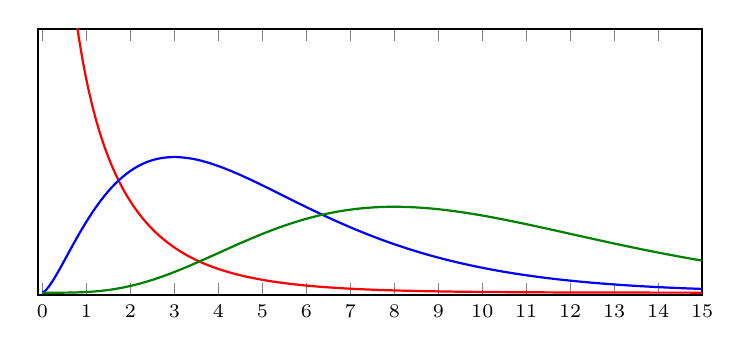
\begin{tikzpicture}[scale = 1]
  \begin{axis}[
  	  scale only axis,
      unit vector ratio=1 20 1,
      ymin=-0.0025,
      ymax=0.3,
      xmin=-0.1,
      xmax=15,
      tick label style={font=\scriptsize, scale = 1/1},
      xtick={0,1,2,3,4,5,6,7,8,9,10,11,12,13,14,15},
      ytick=\empty,
      legend pos=north east,
      domain=0:15,
      samples=200,
      thick
    ]
    % Chi-square with 1 degree of freedom
    \addplot[red] {1/(sqrt(2*pi*x))*exp(-x/2)};

    % Chi-square with 5 degrees of freedom
    \addplot[blue]  {1/(pow(2,2.5)*1.32934)*pow(x,1.5)*exp(-x/2)};

    % Chi-square with 10 degrees of freedom
    \addplot[green!50!black]  {1/(pow(2,5)*24)*pow(x,4)*exp(-x/2)};
  \end{axis}
\end{tikzpicture}
\end{center}

\begin{proposition}\label{ChiSquareNullDist}
Consider a random sample of $n$ values from a given discrete distribution which takes $k$ possible values. Let $\mathcal{O}_i$ be the number of times the $i^{th}$ value occurs in the sample, and let $E_i$ be $n$ times the probability of observing the $i^{th}$ value. Then as $n \to \infty$ the distribution of the statistic 
$$\sum_{i=1}^k \frac{(\mathcal{O}_i - E_i)^2}{E_i}$$
approaches the chi-square distribution with $k-1$ degrees of freedom.
\end{proposition}

The proof of this fact is beyond the scope of this course, and appears in more advanced texts \cite{vanderVaart}. It was first shown in 1900 by the statistician Karl Pearson, which is why the test we're about to perform bears his name. Now that we know the distribution of the statistic we computed, which we'll now call $\chi^2 = 5.44$, under the hypothesis that the die is fair, we can carry out a hypothesis test, as we did in the last few sections.

\begin{example}
A die, which may or may not be fair, is rolled fifty times. The results are 8 ones, 4 twos, 11 threes, 6 fours, 9 fives, and 12 sixes (the observed values in the table on the last page). Can we conclude the die is not fair, at the 5\% significance level?

\begin{enumerate}[label=\textnormal{\Roman*}.]
\item $H_0: \text{The die is fair}$, $H_a: \text{The die is not fair}$.

\item Our test statistic is $\chi^2 = \sum_{i=1}^6 \frac{(\mathcal{O}_i - E_i)^2}{E_i} = \frac{(8-\frac{50}{6})^2}{\frac{50}{6}} + \frac{(4-\frac{50}{6})^2}{\frac{50}{6}} + \dots + \frac{(12-\frac{50}{6})^2}{\frac{50}{6}} = 5.44.$ \\

The P-value is the probability of obtaining a sample whose test statistic is at least as large as the one we observed (the larger the $\chi^2$ value, the farther the observed counts are from the expected counts). Thus, the P-value is $P(\chi^2 \geq 5.44)$, i.e., the probability a chi-square random variable with 5 degrees of freedom takes a value greater than or equal to $5.44$.
\begin{center}
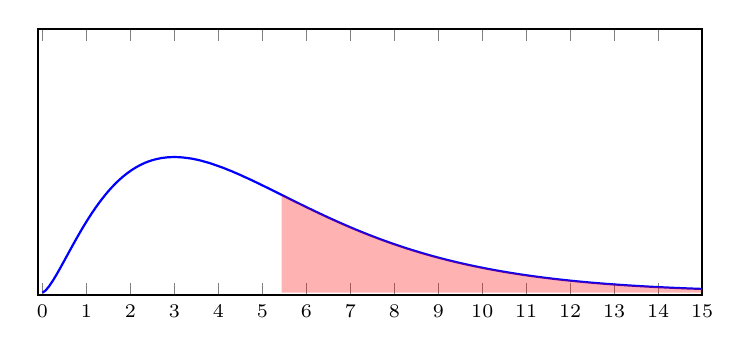
\begin{tikzpicture}[scale = 1]
  \begin{axis}[
  	  scale only axis,
      unit vector ratio=1 20 1,
      ymin=-0.0025,
      ymax=0.3,
      xmin=-0.1,
      xmax=15,
      tick label style={font=\scriptsize, scale = 1/1},
      xtick={0,1,2,3,4,5,6,7,8,9,10,11,12,13,14,15},
      ytick=\empty,
      legend pos=north east,
      domain=0:15,
      samples=200,
      thick
    ]

    % Chi-square with 5 degrees of freedom
    \addplot[blue]  {1/(pow(2,2.5)*1.32934)*pow(x,1.5)*exp(-x/2)};
    
    \addplot[blue, opacity=0, fill=red, fill opacity=0.3, domain=5.44:15] 
      {1/(pow(2,2.5)*1.32934)*pow(x,1.5)*exp(-x/2)} \closedcycle;

  \end{axis}
\end{tikzpicture}
\end{center}
Consulting a table of values for the chi-square distribution, we can find the critical value which produces a tail area of 5\% is about 11. Therefore, the P-value in our test is (much) larger than 5\%. Using a computer to explicitly compute the area gives $P = 0.366$.

\item Since $P > 0.05$, we have not seen sufficient evidence to conclude that the die is not fair, at the 5\% significance level.
\end{enumerate}
\end{example}

This test can be used in many scenarios where we want to know whether some treatment results in a change from a known distribution, and is usually known as the \newterm{chi-square goodness-of-fit test}\index{Pearson's Chi-Square Test! for Goodness of Fit}. It attempts to answer the very general question: could this sample have come from that distribution?

For example, from past data, we may know the distribution of the number of weeks it takes patients to fully recover from a certain surgery. If adding physiotherapy sessions has no effect on recovery time, the recovery times in a sample of patients who undergo physiotherapy is a sample from this same distribution (the null hypothesis of the test), and if the physiotherapy is actually having some kind of effect, it's a sample from some other distribution (the alternative hypothesis of the test).

\subsection*{Testing Independence}

We can use a variation of this test, the \newterm{chi-square test of independence}\index{Pearson's Chi-Square Test! of Independence}, to check for evidence that two variables are not independent in a given population. Suppose we ask a random sample of 109 people at the college, all of whom are in their twenties, thirties, or fourties, whether they prefer to drink tea or coffee. The number of individuals in the sample who fall into each possible category of age and drink preference is given in the table below.
\renewcommand{\arraystretch}{1.25}
\begin{center}
\begin{tabular}{|c|c|c|c|c|c|c|}
\hline
 & Twenties & Thirties & Fourties \\
\hline
Prefer Tea & $17$ & $7$ & $10$  \\
\hline
Prefer Coffee & $23$ & $25$ & $27$ \\
\hline
\end{tabular}
\end{center}

Notice that there are finitely many categories into which values of each variable can belong. We'll add the totals along each row and column, as well as the grand total of all six values in the bottom right. The result is known as a \newterm{contingency table}\index{Contingency Table}.
\renewcommand{\arraystretch}{1.25}
\begin{center}
\begin{tabular}{|c|c|c|c|c|c|c|}
\hline
 & Twenties & Thirties & Fourties & Total \\
\hline
Prefer Tea & $17$ & $7$ & $10$ & $34$  \\
\hline
Prefer Coffee & $23$ & $25$ & $27$ & $75$ \\
\hline
Total & $40$ & $32$ & $37$  & $109$ \\
\hline
\end{tabular}
\end{center}

Now suppose that we only had the row and column totals, but we knew that age and drink preference were independent variables.
\renewcommand{\arraystretch}{1.25}
\begin{center}
\begin{tabular}{|c|c|c|c|c|c|c|}
\hline
 & Twenties & Thirties & Fourties & Total \\
\hline
Prefer Tea & $?$ & $?$ & $?$ & $34$  \\
\hline
Prefer Coffee & $?$ & $?$ & $?$ & $75$ \\
\hline
Total & $40$ & $32$ & $37$  & $109$  \\
\hline
\end{tabular}
\end{center}

Since the probability a randomly selected individual prefers tea and is in their twenties is the product of the probability they prefer tea and the probability they are in their twenties (that is the definition of independence), we can compute the number of individuals who prefer tea and are in their twenties we would expect to see in our sample as $P(\text{Tea} \cap \text{Twenties}) = \frac{34}{109}\frac{40}{109}$, so the expected number in that cell is $N(\text{Tea} \cap \text{Twenties}) = 109\cdot\frac{34}{109}\cdot\frac{40}{109} = \frac{34\cdot 40}{109} = 12.48$.

In general, if the two variables we measured are independent, the expected count in each cell in the table is the product of the corresponding row and column totals, divided by the grand total, briefly, $E_{i,j} = \frac{R_i \cdot C_j}{n}$. Filling in each entry in this manner gives us the expected counts in our sample under the hypothesis that the two variables are independent.
\renewcommand{\arraystretch}{1.25}
\begin{center}
\begin{tabular}{|c|c|c|c|c|c|c|}
\hline
 & Twenties & Thirties & Fourties & Total \\
\hline
Prefer Tea & $12.75$ & $9.98$ & $11.54$ & $34$  \\
\hline
Prefer Coffee & $27.52$ & $22.02$ & $25.46$ & $75$ \\
\hline
Total & $40$ & $32$ & $37$  & $109$  \\
\hline
\end{tabular}
\end{center}

Computing the chi-square statistic (the weighted sum of the squared differences between the observed and expected counts, each term weighted with its expected count, as before) gives
$$\sum_{i=1}^2\sum_{j=1}^3 \frac{(\mathcal{O}_{i,j} - E_{i,j})^2}{E_{i,j}} = \frac{(17-12.75)^2}{12.75} + \frac{(7-9.98)^2}{9.98} + \dots + \frac{(27-25.46)^2}{25.46} = 3.75.$$

\begin{proposition}
Consider a random sample of $n$ individuals, and two categorical variables $X$ and $Y$ which can take $r$ and $c$ possible values respectively in the population. Let $\mathcal{O}_{i,j}$ be the number of times the $i^{th}$ value of $X$ occurs together with the $j^{th}$ value of $Y$ in the sample, and let $E_{i,j} = \frac{R_i \cdot C_j}{n}$, where $R_i$ is the total number of times the $i^{th}$ value of $X$ occurs in the sample, and $C_j$ is the total number of times the $j^{th}$ value of $Y$ occurs in the sample. If the variables $X$ and $Y$ are independent in the population, then as $n \to \infty$ the distribution of the statistic 
$$\sum_{i=1}^r\sum_{j=1}^c \frac{(\mathcal{O}_{i,j} - E_{i,j})^2}{E_{i,j}}$$
approaches the chi-square distribution with $(r-1)(c-1)$ degrees of freedom.
\end{proposition}

As with Proposition \ref{ChiSquareNullDist}, the proof is beyond the scope of this course, but it's possible to give an intuitive interpretation of the number of degrees of freedom. Given fixed row and column totals in a contingency table with $r$ rows and $c$ columns, $(r-1)(c-1)$ is precisely the number of entries that need to be specified to determine the table completely. 

Consider a $2 \times 2$ contingency table, for example, with fixed row and column totals. Once any single value is specified, the other entry in the same row can be obtained by subtracting that value from the row total. At that point, each column has one entry fixed, and the other can be obtained by subtracting it from the respective column total. This means that only a single entry in the table can be freely chosen, and once that's done, the rest are completely determined, hence $(2-1)(2-1) = 1$ degree of freedom. This reasoning generalizes to larger tables as well.

With the distribution of the chi-square statistic under the hypothesis that the variables are independent established, we can perform the hypothesis test in the usual framework of this chapter.

\begin{example}
A random sample of 109 people at a college, all of whom are in their twenties, thirties, or fourties, are asked whether they prefer to drink tea or coffee. The number of individuals in the sample who fall into each possible category of age and drink preference is given in the table below. Can we conclude that age and drink preference are not independent variables, at the 10\% significance level?
\renewcommand{\arraystretch}{1.25}
\begin{center}
\begin{tabular}{|c|c|c|c|c|c|c|}
\hline
 & Twenties & Thirties & Fourties \\
\hline
Prefer Tea & $17$ & $7$ & $10$  \\
\hline
Prefer Coffee & $23$ & $25$ & $27$ \\
\hline
\end{tabular}
\end{center}

We begin by constructing the contingency table, summing along each row and column, as above, and then compute the expected count in each cell. The results are given below.
\renewcommand{\arraystretch}{1.25}
\begin{center}
\begin{tabular}{|c|c|c|c|c|c|c|}
\hline
 & Twenties & Thirties & Fourties & Total \\
\hline
Prefer Tea & $12.75$ & $9.98$ & $11.54$ & $34$  \\
\hline
Prefer Coffee & $27.52$ & $22.02$ & $25.46$ & $75$ \\
\hline
Total & $40$ & $32$ & $37$  & $109$  \\
\hline
\end{tabular}
\end{center}

\begin{enumerate}[label=\textnormal{\Roman*}.]
\item $H_0: \text{Age and drink preference are independent}$, $H_a: \text{Age and drink preference are not independent}$.

\item Our test statistic is $\chi^2 = \sum_{i=1}^2\sum_{j=1}^3 \frac{(\mathcal{O}_{i,j} - E_{i,j})^2}{E_{i,j}} = \frac{(17-12.75)^2}{12.75} + \frac{(7-9.98)^2}{9.98} + \dots + \frac{(27-25.46)^2}{25.46} = 3.75.$ \\

The P-value is the probability of obtaining a sample whose test statistic is at least as large as the one we observed (the larger the $\chi^2$ value, the farther the observed counts are from the expected counts). Thus, the P-value is $P(\chi^2 \geq 3.75)$, i.e., the probability a chi-square random variable with $(2-1)(3-1) = 2$ degrees of freedom takes a value greater than or equal to $3.75$.
\begin{center}
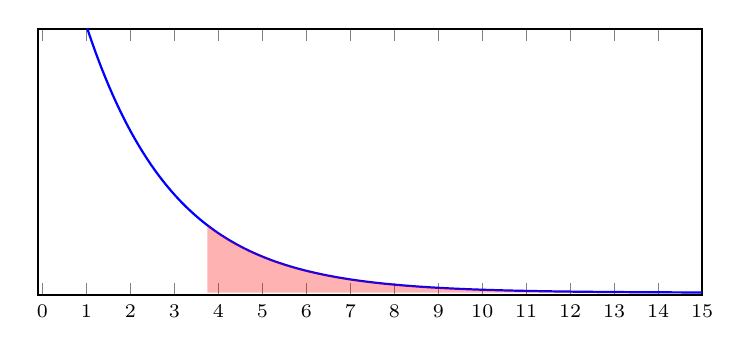
\begin{tikzpicture}[scale = 1]
  \begin{axis}[
  	  scale only axis,
      unit vector ratio=1 20 1,
      ymin=-0.0025,
      ymax=0.3,
      xmin=-0.1,
      xmax=15,
      tick label style={font=\scriptsize, scale = 1/1},
      xtick={0,1,2,3,4,5,6,7,8,9,10,11,12,13,14,15},
      ytick=\empty,
      legend pos=north east,
      domain=0:15,
      samples=200,
      thick
    ]

    % Chi-square with 5 degrees of freedom
    \addplot[blue]  {(1/2)*exp(-x/2)};
    
    \addplot[blue, opacity=0, fill=red, fill opacity=0.3, domain=3.75:15] 
      {(1/2)*exp(-x/2)} \closedcycle;

  \end{axis}
\end{tikzpicture}
\end{center}
Consulting a table of values for the chi-square distribution, we can find the critical value which produces a tail area of 10\% is about $4.605$. Therefore, the P-value in our test is (much) larger than 10\%. Using a computer to explicitly compute the area gives $P = 0.153$.

\item Since $P > 0.10$, we have not seen sufficient evidence to conclude that age and drink preference are not independent, at the 10\% significance level.
\end{enumerate}
\end{example}

\begin{remark}
We're testing how far our sample data is from what we would expect to see if the variables were independent. Either we have seen enough evidence to convince us they are not, or we haven't seen enough evidence to convince us they are not. We can never conclude the variables are independent from sample data.
\end{remark}

\begin{example}
A biologist crosses pea plants to examine the distribution of two traits in the offspring, seed shape (round or wrinkled) and seed colour (yellow or green). The resulting number of plants with each combination of traits is given below.
\renewcommand{\arraystretch}{1.25}
\begin{center}
\begin{tabular}{|c|c|c|c|c|c|c|}
\hline
 & Yellow & Green \\
\hline
Round & $29$ & $9$  \\
\hline
Wrinkled & $11$ & $11$ \\
\hline
\end{tabular}
\end{center}

If there is no genetic linkage between the genes that code for the two traits, we would expect the two variables to be independent (whether one is inherited does not change the probability of inheriting the other). Does this sample provide enough evidence, at the 5\% significance level, to conclude otherwise? 

We begin by finding the row and column totals, and computing the expected count in each cell.
\renewcommand{\arraystretch}{1.25}
\begin{center}
\begin{tabular}{|c|c|c|c|c|c|c|}
\hline
 & Yellow & Green & Total \\
\hline
Round & $25.33$ & $12.67$ & $38$ \\
\hline
Wrinkled & $14.67$ & $7.33$ & $22$ \\
\hline
Total & $40$ & $20$ & $60$ \\
\hline
\end{tabular}
\end{center}

\begin{enumerate}[label=\textnormal{\Roman*}.]
\item $H_0: \text{Seed shape and colour and are inherited independently (i.e. not linked)}$ \\
$H_a: \text{Seed shape and colour and are not inherited independently (i.e. linked)}$.

\item Our test statistic is $\chi^2 = \sum_{i=1}^2\sum_{j=1}^2 \frac{(\mathcal{O}_{i,j} - E_{i,j})^2}{E_{i,j}} = \frac{(29-25.33)^2}{25.33} + \frac{(9-12.67)^2}{12.67} + \dots + \frac{(11-7.33)^2}{7.33} = 4.35.$ \\

The P-value is the probability of obtaining a sample whose test statistic is at least as large as the one we observed, i.e., the probability a chi-square random variable with $(2-1)(2-1) = 1$ degree of freedom takes a value greater than or equal to $4.35$.
\begin{center}
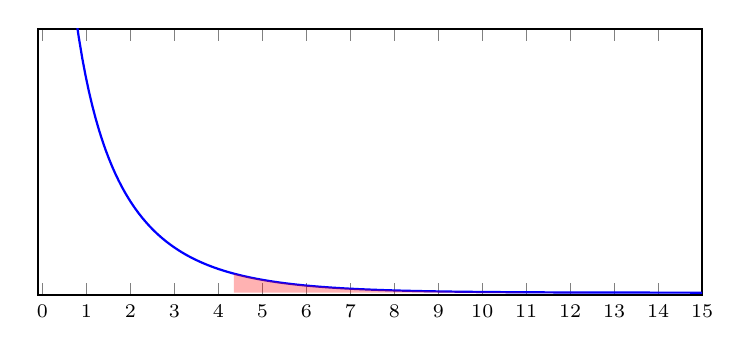
\begin{tikzpicture}[scale = 1]
  \begin{axis}[
  	  scale only axis,
      unit vector ratio=1 20 1,
      ymin=-0.0025,
      ymax=0.3,
      xmin=-0.1,
      xmax=15,
      tick label style={font=\scriptsize, scale = 1/1},
      xtick={0,1,2,3,4,5,6,7,8,9,10,11,12,13,14,15},
      ytick=\empty,
      legend pos=north east,
      domain=0:15,
      samples=200,
      thick
    ]

    % Chi-square with 5 degrees of freedom
    \addplot[blue]  {(1/pow(2*pi*x,0.5))*exp(-x/2)};
    
    \addplot[blue, opacity=0, fill=red, fill opacity=0.3, domain=4.35:15] 
      {(1/pow(2*pi*x,0.5))*exp(-x/2)} \closedcycle;

  \end{axis}
\end{tikzpicture}
\end{center}
Consulting a table of values for the chi-square distribution, we can find the critical value which produces a tail area of 5\% is $3.841$. Therefore, the P-value in our test is smaller than 5\%. Using a computer to explicitly compute the area gives $P = 0.037$.

\item Since $P < 0.05$, we can conclude that seed shape and colour are not inherited independently, i.e., are linked, at the 5\% significance level.
\end{enumerate}
\end{example}

\begin{remark}
In fact, seed shape and colour in pea plants are inherited independently (this is a classic example in genetics), so in the test above a Type I error occurred. We rejected a true null hypothesis, which is what will occur in 5\% of samples.

The point to remember is that 95\% of the time, when the experiment is performed, the test will not achieve significance, so the balance of evidence will lead us to the correct conclusion.
\end{remark}

%\begin{example} In the United States, 8\% of families do not have a car, 33\% have one car, 38\% have two, 14\% have three, and 7\% have four or more. In a survey of a random sample of 210 Canadian families, 23 did not have a car, 81 had one car, 75 had two, 24 had three, and 7 had four or more.

%Is this sufficient evidence to conclude, at the 10\% significance level, that the distribution of the number of cars per family differs between the two countries?

%\renewcommand{\arraystretch}{1.25}
%\begin{center}
%\begin{tabular}{|c|c|c|c|c|c|c|}
%\hline
%Number of Cars & $0$ & $1$ & $2$ & $3$ & $> 3$ \\
%\hline
%Observed Count & $23$ & $81$ & $75$ & $24$ & $7$ \\
%\hline
%Expected Count & $210 \cdot 0.08$ & $210 \cdot 0.33$ & $210 \cdot 0.38$ & $210 \cdot 0.14$  & $210 \cdot 0.07$   \\
%\hline
%\end{tabular}
%\end{center}

%\begin{enumerate}[label=\textnormal{\Roman*}.]
%\item $H_0: \text{The distributions are identical}$, $H_a: \text{The distributions differ between countries}$.

%\item Our test statistic is $\chi^2 = \sum_{i=1}^5 \frac{(\mathcal{O}_i - E_i)^2}{E_i} = \frac{(23-16.8)^2}{16.8} + \frac{(81-69.3)^2}{69.3} + \dots + \frac{(7-14.7)^2}{14.7} = 9.58$

%The P-value is the probability a $\chi^2$ random variable with 4 degrees of freedom takes a value greater than 9.58, i.e., $P(\chi^2 \geq 9.58)$.
%\begin{center}
%\begin{tikzpicture}[scale = 1]
%  \begin{axis}[
%  	  scale only axis,
%      unit vector ratio=1 20 1,
%      ymin=-0.0025,
%      ymax=0.3,
%      xmin=-0.1,
%      xmax=15,
%      tick label style={font=\scriptsize, scale = 1/1},
%      xtick={0,1,2,3,4,5,6,7,8,9,10,11,12,13,14,15},
%      ytick=\empty,
%      legend pos=north east,
%      domain=0:15,
%      samples=200,
%      thick
%    ]
%
%    % Chi-square with 4 degrees of freedom
%    \addplot[blue]  {1/(pow(2,2)*1)*pow(x,1)*exp(-x/2)};
%    
%    \addplot[blue, opacity=0, fill=red, fill opacity=0.3, domain=9.58:15] 
%      {1/(pow(2,2)*1)*pow(x,1)*exp(-x/2)} \closedcycle;
%
%  \end{axis}
%\end{tikzpicture}
%\end{center}
%Consulting a table of values for the chi-square distribution, we can find the critical value which produces a tail area of 10\% is 7.78. Therefore, the P-value in our test is smaller than 10\%. Using a computer to explicitly compute the area gives $P = 0.048$.

%\item Since $P < 0.10$, we have seen sufficient evidence to conclude that the distribution of number of cars per family is different in the two countries, at the 10\% significance level.

%\end{enumerate}
%\end{example}

%\begin{remark}
%There's a variation of this test used to assess whether enough evidence is present in a set of sample data to conclude that two variables are not independent. That variation is usually called the chi-square test of independence, while the test developed in this section is known as the chi-square goodness-of-fit test.
%\end{remark}





